%=============================================================================
%  Rapport de fin de stage
%  Projet : Simulateur de controleur aerien -- copilote IA pour le controle aerien
%  Auteur : Nicolas Marano -- URCA / supercalculateur ROMEO (NVIDIA GH200)
%  Compilation : pdflatex (x2 pour la table des matieres) -- via WSL
%=============================================================================
\documentclass[11pt,a4paper]{article}

\usepackage[utf8]{inputenc}
\usepackage[T1]{fontenc}
\usepackage[french]{babel}
\usepackage{lmodern}
\usepackage{microtype}
\usepackage[a4paper,margin=2.3cm,headheight=15pt]{geometry}
\usepackage{graphicx}
\usepackage{booktabs}
\usepackage{array}
\usepackage[table]{xcolor}
\usepackage{titlesec}
\usepackage{enumitem}
\usepackage{caption}
\usepackage{fancyhdr}
\usepackage{listings}
\usepackage[most]{tcolorbox}
\usepackage{amsmath}
\usepackage{tikz}
\usetikzlibrary{positioning,arrows.meta,shapes.geometric,fit}
\usepackage{placeins}
\usepackage{hyperref}

%--- Couleurs ----------------------------------------------------------------
\definecolor{atcblue}{RGB}{11,61,145}
\definecolor{atcteal}{RGB}{13,110,124}
\definecolor{atcgreen}{RGB}{22,128,71}
\definecolor{atcred}{RGB}{197,32,38}
\definecolor{atcpurple}{RGB}{109,40,180}
\definecolor{atcslate}{RGB}{71,85,105}
\definecolor{lightgray}{RGB}{244,246,249}
\definecolor{rulegray}{RGB}{210,216,224}

\hypersetup{colorlinks=true, linkcolor=atcblue, urlcolor=atcteal, citecolor=atcblue,
  pdftitle={Rapport de fin de stage -- Copilote IA pour le controle aerien},
  pdfauthor={Nicolas Marano}}

%--- Titres ------------------------------------------------------------------
\titleformat{\section}{\Large\bfseries\color{atcblue}}{\thesection}{0.6em}{}
\titleformat{\subsection}{\large\bfseries\color{atcteal}}{\thesubsection}{0.6em}{}
\titleformat{\subsubsection}{\normalsize\bfseries\color{atcteal}}{\thesubsubsection}{0.5em}{}
\titlespacing*{\section}{0pt}{16pt}{8pt}

%--- En-tete / pied de page --------------------------------------------------
\pagestyle{fancy}
\fancyhf{}
\renewcommand{\headrulewidth}{0.4pt}
\renewcommand{\footrulewidth}{0.4pt}
\fancyhead[L]{\small\color{atcblue}\itshape Copilote IA pour le contrôle aérien}
\fancyhead[R]{\small\color{atcblue}\itshape Rapport de fin de stage}
\fancyfoot[L]{\small Nicolas Marano, URCA / ROMEO}
\fancyfoot[R]{\small\thepage}

%--- Boites tcolorbox --------------------------------------------------------
\newtcolorbox{objbox}[1][Objectif]{enhanced, colback=lightgray, colframe=atcblue,
  boxrule=0.8pt, arc=3pt, left=10pt, right=10pt, top=8pt, bottom=8pt,
  fonttitle=\bfseries\color{white}, coltitle=white, colbacktitle=atcblue,
  title={#1}}

\newtcolorbox{resbox}[1][Résultats clés]{enhanced, colback=atcgreen!6, colframe=atcgreen,
  boxrule=0.8pt, arc=3pt, left=10pt, right=10pt, top=8pt, bottom=8pt,
  fonttitle=\bfseries, coltitle=white, colbacktitle=atcgreen,
  title={#1}}

\newtcolorbox{warnbox}[1][Difficultés rencontrées et résolutions]{enhanced, colback=atcslate!6, colframe=atcslate,
  boxrule=0.8pt, arc=3pt, left=10pt, right=10pt, top=8pt, bottom=8pt,
  fonttitle=\bfseries, coltitle=white, colbacktitle=atcslate,
  title={#1}}

%--- Style des listings ------------------------------------------------------
\lstdefinestyle{atccode}{
  basicstyle=\ttfamily\footnotesize,
  backgroundcolor=\color{lightgray},
  frame=single, framesep=5pt, rulecolor=\color{rulegray},
  breaklines=true, breakatwhitespace=true,
  showstringspaces=false,
  keywordstyle=\color{atcblue}\bfseries,
  commentstyle=\color{atcgreen}\itshape,
  stringstyle=\color{atcpurple},
  numberstyle=\tiny\color{gray},
  columns=fullflexible, keepspaces=true,
  aboveskip=8pt, belowskip=8pt,
}
\lstset{style=atccode}

\setlist[itemize]{label=\textbullet, leftmargin=1.4em, itemsep=2pt, topsep=3pt}
\captionsetup{font=small, labelfont={bf,color=atcblue}}
\renewcommand{\arraystretch}{1.25}

%=============================================================================
\begin{document}

%--- Page de garde -----------------------------------------------------------
\begin{titlepage}
\centering
\vspace*{1.0cm}
{\color{atcblue}\rule{\textwidth}{2pt}}\\[0.5cm]
{\Huge\bfseries\color{atcblue} Rapport de fin de stage\par}
\vspace{0.35cm}
{\LARGE\color{atcteal} Un copilote d'intelligence artificielle\\pour le contrôle du trafic aérien\par}
\vspace{0.25cm}
{\large Parler aux avions, et que les avions répondent : choix scientifiques,\\[2pt] obstacles d'ingénierie et validation expérimentale de la chaîne vocale STT $\rightarrow$ LLM $\rightarrow$ TTS\par}
\vspace{0.4cm}
{\color{atcblue}\rule{\textwidth}{2pt}}\\[0.9cm]

\begin{tabular}{rl}
\large\bfseries Auteur & \large Nicolas Marano\\[4pt]
\large\bfseries Projet & \large Simulateur de contrôleur aérien (PoC, 10 semaines)\\[4pt]
\large\bfseries Établissement & \large Université de Reims Champagne-Ardenne (URCA)\\[4pt]
\large\bfseries Calcul (IA) & \large Supercalculateur ROMEO : NVIDIA GH200 (Grace-Hopper, aarch64)\\[4pt]
\large\bfseries Domaine & \large Intelligence artificielle \& contrôle du trafic aérien\\[4pt]
\large\bfseries Dépôt & \large \texttt{github.com/Gotman08/simulateur-controleur-aerien}\\
\end{tabular}

\vfill
\begin{tcolorbox}[colback=lightgray, colframe=atcblue, arc=3pt, width=0.94\textwidth, center,
  left=12pt, right=12pt, top=8pt, bottom=8pt]
\small
\textbf{Résumé.} L'objectif premier de ce stage tient en une phrase : permettre à un élève contrôleur de parler à des avions, et que les avions lui répondent. Tout le reste en découle : pour éprouver ce dialogue dans des conditions réalistes, il fallait construire l'environnement complet qui l'entoure, un simulateur d'entraînement au contrôle aérien dont la boucle radio est entièrement pilotée par la voix. La clairance parlée de l'élève est transcrite (Whisper, que j'ai adapté au domaine par LoRA), interprétée en ordres structurés par un grand modèle de langage ancré dans une base de connaissances OACI, filtrée par des gardes déterministes, exécutée dans le simulateur de trafic BlueSky ; l'avion répond alors par un collationnement prononcé dans une voix de synthèse dégradée canal radio VHF. Dans ce rapport final, je justifie mes choix scientifiques au regard de l'état de l'art (pourquoi ces corpus, ces modèles, ces articles plutôt que d'autres), je raconte les difficultés rencontrées et la manière dont je les ai résolues, et j'apporte la preuve mesurée de ce qui fonctionne, et de ce qui ne fonctionne pas. Chiffres clés :
WER de 71,9\,\% $\rightarrow$ 28,5\,\% par adaptation LoRA sur audio VHF réel (gain
significatif, bootstrap apparié) ; 81,9\,\% d'exactitude d'interprétation pour le meilleur
LLM local sur 116 clairances annotées (comparaison appariée de 4 modèles, tests de McNemar) ;
$10^6$ décisions de conflit sans désaccord avec une vérité numérique indépendante et
$F_1 = 1{,}0$ face à BlueSky ; boucle vocale complète à 76\,\% de réussite pour 2,6~s de latence moyenne sur GPU grand public, confirmée par une contre-épreuve avec un locuteur humain réel (80\,\%). L'ensemble du banc de mesure est versionné, seedé et re-exécutable à l'identique.
\end{tcolorbox}
\vspace{0.4cm}
{\small Année universitaire 2025--2026}
\end{titlepage}

%--- Table des matieres ------------------------------------------------------
\tableofcontents
\thispagestyle{fancy}
\clearpage

%=============================================================================
\section{Introduction : contexte, mission et démarche}
%=============================================================================

\subsection{Le problème métier}

Un élève contrôleur s'installe en salle de simulation. Face à lui, un scope radar et une dizaine d'étiquettes qui avancent en temps réel ; dans son casque, le grésillement d'une radio VHF et des pilotes qu'il doit séparer, séquencer et guider dans l'anglais codifié de l'OACI. Deux avions convergent : il a quelques dizaines de secondes pour percevoir le conflit, choisir une man\oe uvre et la transmettre sans ambiguïté. Pour que cette scène fonctionne, il faut aujourd'hui des \emph{pseudo-pilotes} : des opérateurs humains qui, derrière la cloison, prononcent les collationnements et exécutent chaque instruction de l'élève dans le simulateur.

Ce facteur humain domine le coût d'exploitation des simulateurs de formation. De là vient l'objectif premier de mon stage, facile à énoncer, beaucoup moins à réaliser : que l'élève puisse parler aux avions, et que les avions lui répondent, sans opérateur derrière la cloison. Le rôle à remplacer est difficile pour les modèles de fondation : comprendre une clairance parlée, l'exécuter fidèlement, la collationner d'une voix réaliste, alors que la phraséologie OACI est un langage contraint, que le canal radio VHF (bande utile 300--3\,400~Hz) dégrade fortement le signal, et que toute erreur d'interprétation exécutée dans le simulateur fausse l'exercice pédagogique. Derrière la boucle vocale de 2,6~secondes mesurée à la fin de ce rapport, il y a donc un outil concret, conçu pour des humains en formation.

\subsection{La mission et la chaîne cible}

Le c\oe ur de ma mission, durant ces dix semaines (un PoC encadré par l'URCA), était donc ce dialogue vocal bidirectionnel : l'élève parle, l'avion man\oe uvre et répond. Mais un dialogue ne se teste pas dans le vide : pour que l'avion ait un ordre à exécuter et un état à collationner, il faut un trafic simulé, un espace aérien, un radar. C'est ce qui m'a conduit à construire et évaluer toute la chaîne suivante, avec les modèles d'IA hébergés sur le supercalculateur ROMEO (n\oe ud GH200 Grace-Hopper, aarch64, 96~Go) et le simulateur sur un poste local :

\begin{center}
\fbox{\parbox{0.95\textwidth}{\centering\ttfamily\footnotesize
voix contrôleur (VHF) $\rightarrow$ Whisper STT $\rightarrow$ NER + LLM ancré (base OACI, graphe secteur)
$\rightarrow$ JSON validé\\
$\rightarrow$ simulateur BlueSky (man\oe uvre) $\rightarrow$ collationnement en voix de synthèse VHF $\rightarrow$ boucle}}
\end{center}

Le livrable auquel j'ai abouti dépasse le PoC initial : une application web d'entraînement complète (scope radar 60~fps, strips, poste instructeur en langage naturel, mode exercice noté avec débriefing, figure~\ref{fig:app}), adossée à une campagne de validation mathématique et empirique et à un banc de mesure scientifique versionné avec le code. Il faut toutefois garder la hiérarchie en tête : radar, exercices et simulateur ne sont que l'infrastructure de test ; tout le projet se joue dans l'échange radio entre l'élève et l'avion.

\begin{figure}[h]
\centering
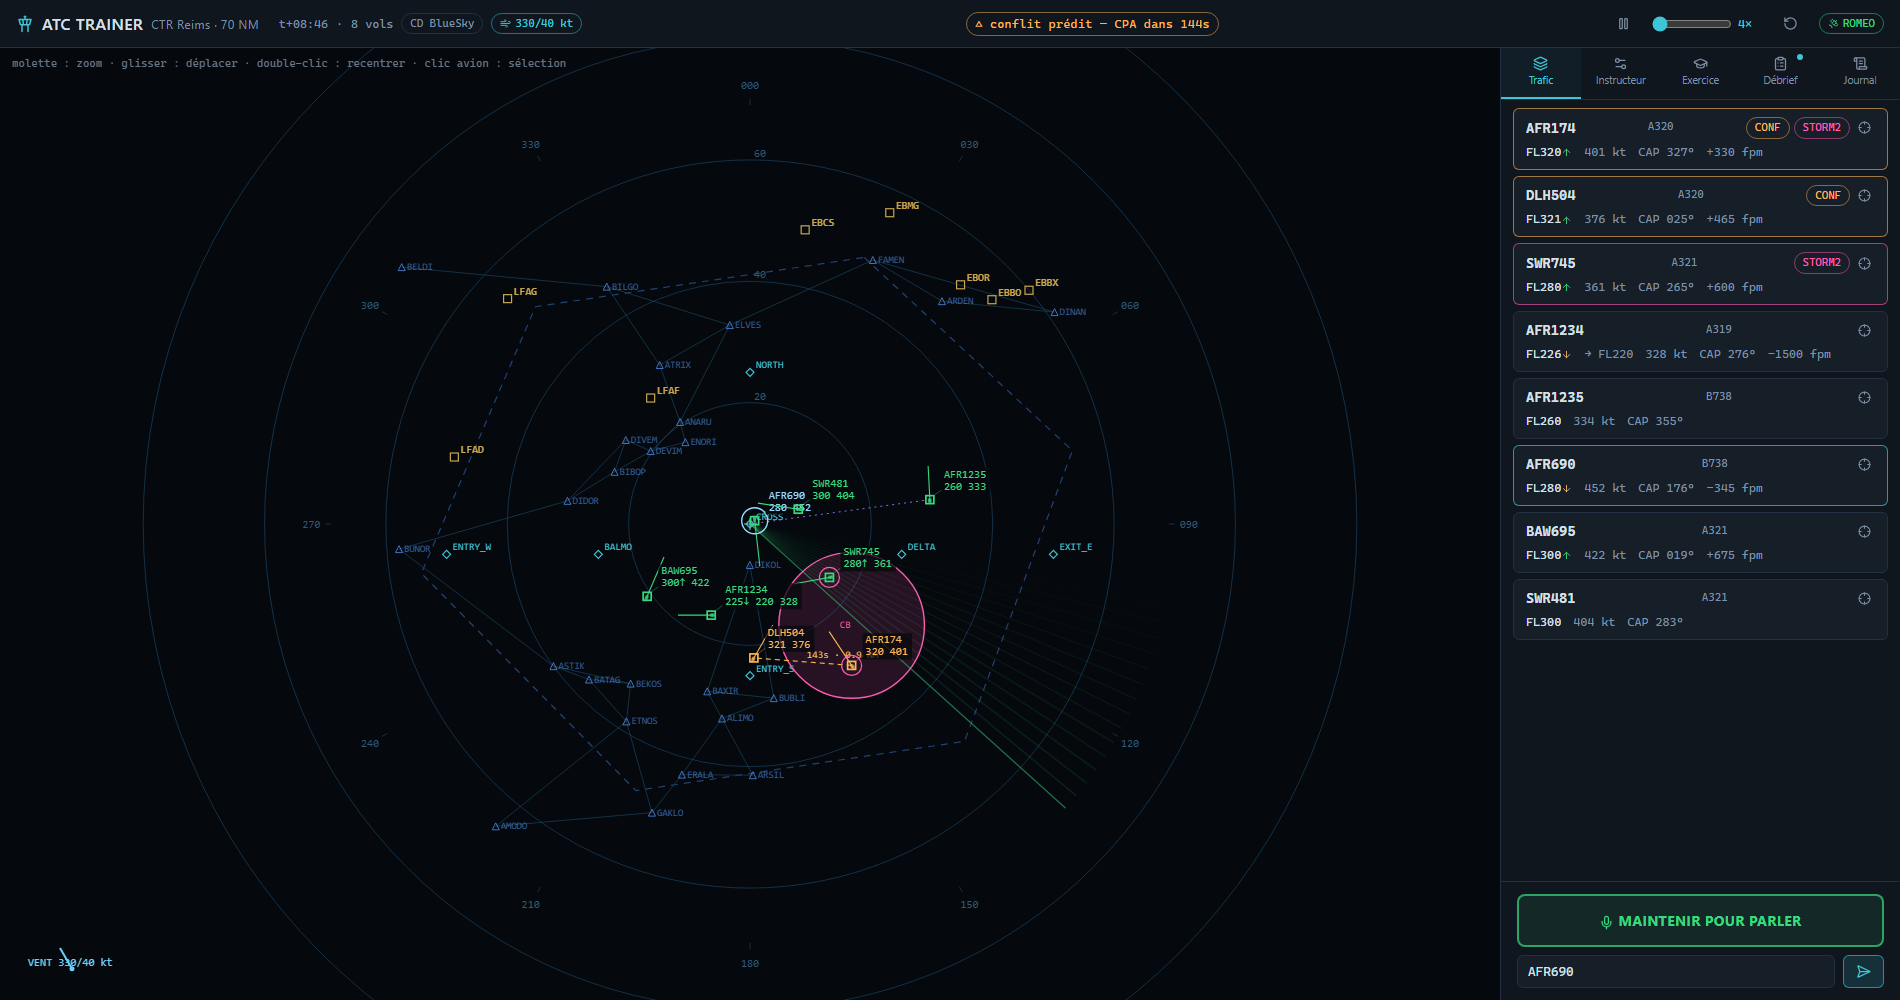
\includegraphics[width=0.9\textwidth]{figures/app_radar.png}
\caption{L'application d'entraînement livrée : scope radar temps réel (BlueSky), strips de
vol, poste instructeur et position contrôleur \emph{push-to-talk}.}
\label{fig:app}
\end{figure}

\subsection{Organisation du rapport}

J'ai organisé ce document autour de trois questions : \textbf{(i)} pourquoi mes choix scientifiques (articles de référence, corpus, modèles, simulateur) plutôt que leurs alternatives (section~\ref{sec:etat-art}) ; \textbf{(ii)} quelles difficultés j'ai rencontrées et comment je les ai résolues, preuves à l'appui (section~\ref{sec:problemes}) ; \textbf{(iii)} ce que je considère comme \emph{prouvé}, avec quelles limites documentées (sections~\ref{sec:validation} et \ref{sec:limites}). La section~\ref{sec:realisation} décrit au préalable comment j'ai construit le système, phase par phase.

%=============================================================================
\section{État de l'art et justification des choix scientifiques}
\label{sec:etat-art}
%=============================================================================

\begin{objbox}[Démarche de sélection bibliographique]
J'ai constitué l'état de l'art en semaines 1 et 2 (\texttt{src/references.bib}) selon quatre critères explicites : \textbf{(a)} priorité aux travaux s'appuyant sur des
\emph{données radio réelles} plutôt que sur des données de laboratoire ; \textbf{(b)}
reproductibilité (corpus publics, poids ouverts, code disponible) ; \textbf{(c)}
compatibilité avec les contraintes matérielles du stage (cluster aarch64, quota disque de
20~Go par partition, 10 semaines, exécution locale possible) ; \textbf{(d)} actualité
(2022--2026, le domaine évoluant très vite). Chaque choix retenu ci-dessous est confronté à ses alternatives, puis \emph{validé a posteriori par une mesure}. C'est le fil conducteur de mon travail : je n'ai laissé aucune décision d'architecture reposer sur la seule autorité d'un article.
\end{objbox}

\subsection{Corpus de parole ATC : pourquoi ATCO2, UWB-ATCC et ATCOSIM}
\label{sec:corpus}

Le choix des données d'entraînement conditionne tout l'étage de reconnaissance vocale. Avant de retenir les corpus de la communauté ATCO2, j'ai examiné puis écarté trois familles d'alternatives. La collecte directe de flux LiveATC fournit du volume, mais \emph{sans transcriptions} et avec un statut juridique incertain ; inutilisable telle quelle pour un apprentissage supervisé en 10 semaines. Les corpus propriétaires des prestataires de navigation aérienne sont de meilleure qualité, mais inaccessibles dans le cadre du stage et non reproductibles par un tiers. Restaient les données synthétiques (TTS), disponibles à volonté, mais qui introduisent un écart de domaine (\emph{sim-to-real}) précisément là où le projet cherche de la robustesse au canal réel.

Le triplet que j'ai retenu est issu des travaux de la communauté ATCO2~\cite{atco2,uwbatcc,atcosim}, qui a établi la reconnaissance vocale ATC comme domaine de recherche à part entière et publié les seuls grands corpus \emph{réels, transcrits et publics} du domaine. Leur complémentarité a dicté mon protocole : UWB-ATCC~\cite{uwbatcc} (radio réelle, bruitée, accents variés) et ATCOSIM~\cite{atcosim} (parole de simulateur, propre) servent à l'\emph{entraînement et à la validation}, le modèle voyant à la fois du canal dégradé et de la parole nette ; ATCO2-1h~\cite{atco2}, l'audio le plus difficile (radio opérationnelle réelle), est \emph{réservé au test} et n'est jamais vu à l'entraînement. Ce choix d'un jeu de test sévère et hors distribution est délibéré : je voulais mesurer la généralisation, pas la mémorisation.

\noindent\textbf{Preuve a posteriori.} Cette stratégie est validée par les mesures : le WER
sur ATCO2 (domaine jamais vu) passe de 71,9\,\% à 28,5\,\% après adaptation
(section~\ref{sec:res-stt}), et l'écart entre le WER de validation (6,68\,\%, domaine
d'entraînement) et le WER de test (28--29\,\%) quantifie exactement le fossé de
généralisation que le protocole était conçu pour révéler.

\subsection{Reconnaissance vocale : pourquoi Whisper, et pourquoi LoRA}

\paragraph{Whisper plutôt qu'une autre famille acoustique.} L'intuition d'abord : inutile d'apprendre à un modèle à écouter depuis zéro quand il en existe un qui a déjà entendu des centaines de milliers d'heures de parole dans des conditions très variées ; il suffit de le spécialiser sur les nôtres. J'ai donc préféré Whisper~\cite{whisper} aux encodeurs auto-supervisés de type wav2vec2 et aux API de transcription commerciales, pour quatre raisons convergentes : (i) son entraînement
faiblement supervisé à très grande échelle lui confère une robustesse au bruit documentée, déterminante sur un canal VHF ; (ii) ses poids sont ouverts, condition de l'adaptation
au domaine et de la reproductibilité ; (iii) il est multilingue (le projet accepte la
phraséologie anglaise \emph{et} française) ; (iv) surtout, deux travaux récents démontrent
spécifiquement sa transférabilité au contrôle aérien : la thèse de van
Doorn~\cite{vandoorn} (TU Delft, 2023) établit la faisabilité de l'application de Whisper à
l'ATC, et Su et Haq~\cite{suhaq} (2026) fournissent un pipeline \emph{économe en données}
directement aligné avec la situation du stage (petit corpus, modèle \texttt{small}, canal
réel). Ce dernier article s'est révélé le plus opérationnel des deux : j'en ai repris le front-end de canal, un passe-bande de Butterworth 300--3\,400~Hz appliqué à l'entraînement \emph{et} à l'inférence (autrement dit, faire entendre au modèle, dès l'apprentissage, le même son étouffé qu'une vraie radio), ainsi qu'une mise en garde d'implémentation sur le couple LoRA / \texttt{input\_features} qui m'a évité une erreur classique (Whisper est un
modèle séquence-à-séquence dont l'encodeur consomme des spectrogrammes, pas des
identifiants de tokens : le collateur doit rembourrer séparément features et labels).

Une API commerciale aurait par ailleurs interdit l'adaptation au domaine, imposé une
dépendance réseau au poste de formation et fait sortir les données ; ces trois points sont
rédhibitoires pour un simulateur d'entraînement déployable hors ligne.

\paragraph{Taille \texttt{small}.} \texttt{whisper-small} (244~M de paramètres) est le compromis que j'ai retenu entre qualité et coût : il tient largement sur le GH200 pour
l'entraînement, et son facteur temps réel d'inférence mesuré (RTF 0,04 sur cluster, 0,017
sur GPU portable) laisse une marge confortable pour la boucle interactive. Les tailles
supérieures auraient allongé les itérations d'entraînement sans lever le goulot réel, la qualité des données du domaine, et les mesures finales confirment que l'adaptation
domine l'effet de taille : le \texttt{small} adapté bat très largement des modèles
génériques de même gabarit (section~\ref{sec:res-stt}).

\paragraph{LoRA plutôt qu'un affinage complet.} L'idée de LoRA~\cite{lora} : au lieu de réécrire le livre, on l'annote dans la marge. Le modèle de base est gelé, et je n'entraîne que de petites matrices correctrices de rang faible ($r = 32$, $\alpha = 64$), insérées dans les projections d'attention \texttt{q\_proj}/\texttt{v\_proj} de l'encodeur et du décodeur. Réentraîner les 244~M de paramètres de \texttt{whisper-small} aurait été instable sur un corpus modeste, et incompatible avec le quota disque de 20~Go du cluster (chaque exécution aurait produit des points de contrôle de plusieurs Go) ; l'adaptateur LoRA, lui, pèse 14~Mo (144 tenseurs), se versionne dans le dépôt git, se distribue et se réverse trivialement. C'est l'approche aujourd'hui dominante pour l'adaptation de Whisper au domaine ATC~\cite{suhaq,vandoorn}.

\subsection{Interprétation : pourquoi un LLM ancré et non affiné, gardé par du déterminisme}
\label{sec:choix-llm}

De tous mes choix d'architecture, c'est le plus structurant. Le principe : au lieu d'apprendre la phraséologie au modèle, je lui mets la documentation sous les yeux au moment de répondre, et je fais vérifier chacune de ses réponses par du code classique qui, lui, ne se trompe jamais sur une borne numérique. Ce choix s'appuie sur une lecture \emph{critique} de trois articles complémentaires.

Zhang et Mott~\cite{zhang} (2024) évaluent les LLM sur la reconstruction de trajectoires de vol et concluent à leur \emph{faiblesse sur les longues séquences de coordonnées numériques brutes}. Cet article m'a servi de contre-exemple fondateur : il proscrit d'injecter l'état brut du trafic (positions, vitesses) dans le prompt. Je fournis à la place au modèle une représentation \emph{symbolique compacte} de l'espace aérien, un graphe de secteur (7 points, 6 segments, séparation 5~NM) résumé en trois lignes de texte, et je laisse tout le calcul géométrique à du code déterministe.

AirTrafficGen~\cite{airtrafficgen} (2025) démontre l'efficacité d'une représentation de l'espace aérien \emph{sous forme de graphe} pour la génération de scénarios de trafic par LLM ; il a directement inspiré le module \texttt{graph\_secteur} (n\oe uds typés entrée/fixe/sortie, arêtes pondérées en NM, Dijkstra pour le routage) et la fonctionnalité << poste instructeur >> où une description en langage naturel devient une situation de trafic.

Sharifi et al.~\cite{sharifi} (2026), enfin, affinent des LLM (SFT puis DPO) pour la déconfliction tactique de drones. J'ai étudié cette voie, \emph{spécialiser le LLM lui-même}, puis je l'ai écartée, pour trois raisons : il n'existe pas de corpus public appariant clairances ATC et commandes exécutables à l'échelle requise par un affinage ; le coût d'itération (10 semaines, quota disque) était incompatible ; enfin, dans un domaine où une erreur exécutée fausse l'exercice, je refusais de faire reposer la sécurité sur des poids appris, par nature non auditables. J'ai donc retenu l'architecture inverse : un modèle généraliste \emph{ancré} (mes 9 fiches de phraséologie inlinées dans le prompt, des indices NER, le graphe de secteur) dont \emph{chaque} sortie traverse une validation déterministe et testée (bornes physiques HDG 0--360$^\circ$ / ALT 0--45\,000~ft / SPD 0--350~kt, actions autorisées, waypoints du secteur, cohérence montée/descente).

\paragraph{Le cas particulier du Doc 4444.} La source normative de la phraséologie est le
Doc 4444 de l'OACI~\cite{icao4444}. Ce document étant protégé, je ne pouvais ni l'ingérer ni le citer verbatim dans une base RAG versionnée : j'ai donc rédigé une base de connaissances \emph{originale} de 9 fiches factuelles ($\sim$2,5~Ko) qui synthétisent les règles (conversions de chiffres, indicatifs en téléphonie,
contextes informatifs à ignorer comme le QNH, règle << en cas de doute, ne rien
produire >>) en intégrant les bornes déjà codées du connecteur BlueSky. La recherche
s'effectue par embeddings \texttt{bge-small-en-v1.5} et similarité cosinus en NumPy pur : un index FAISS aurait ajouté une dépendance lourde sans bénéfice mesurable sur une base de
9 documents.

\paragraph{Preuve a posteriori.} La pertinence de l'approche << généraliste ancré +
gardes >> est démontrée par la campagne comparative (section~\ref{sec:res-llm}) : le
meilleur LLM local atteint 81,9\,\% d'exactitude stricte, \emph{bat le parseur à règles sur
les formulations hors grammaire} (77,1\,\% contre 70,8\,\%), ce qui est précisément sa raison d'être ; et sur les 116 clairances du banc, aucun ordre hors bornes n'a atteint le simulateur, quel que soit le modèle, y compris les plus faibles : la sécurité repose sur les gardes déterministes, non sur le modèle.

\subsection{Simulateur : pourquoi BlueSky}

BlueSky~\cite{bluesky} (TU Delft) est le simulateur de trafic open source de référence de
la recherche ATM. J'ai écarté les alternatives (simulateurs commerciaux fermés, plateformes de type Euroscope orientées contrôle en réseau, développement d'un moteur maison) respectivement pour inaccessibilité, inadaptation au pilotage programmatique, et coût hors de portée d'un PoC. BlueSky offre exactement ce dont ma boucle a besoin : un
mode \emph{headless} pilotable par commandes texte (TrafScript), des modèles de
performances avion réalistes (OpenAP), une détection de conflits native (StateBased), et
une base de code Python inspectable. \textbf{Preuve a posteriori} : le simulateur avance
10~s de trafic avec un facteur temps réel de $\times$105 à 5 aéronefs et encore
$\times$67 à 200 aéronefs (figure~\ref{fig:scaling}), il n'est donc jamais le facteur limitant, et son détecteur de conflits confronté au prédicteur analytique du projet
donne une matrice de confusion parfaite sur 200 rencontres (section~\ref{sec:res-geo}).

\subsection{Synthèse vocale : pourquoi le clonage \emph{zero-shot}, puis Kokoro en local}

Mon cahier des charges imposait une voix \emph{distincte et stable par aéronef}. Entraîner un modèle TTS par locuteur était exclu (ni corpus dédié, ni budget de calcul, ni quota disque) ; j'ai donc retenu XTTS-v2~\cite{xtts} pour sa capacité de clonage \emph{zero-shot} : un
extrait de référence de quelques secondes (tiré du corpus ATCO2, donc au timbre << radio >>
authentique) suffit à produire une voix, sans aucun entraînement. Pour le point de déploiement local, j'ai ensuite ajouté le moteur Kokoro-82M (poids ouverts, ONNX) : pas de
clonage, mais un pool de voix stables (affectation par hachage CRC32 de l'indicatif) et un
facteur temps réel de 0,34 sur GPU portable. Dans les deux cas, la dégradation VHF
(Butterworth d'ordre 6, 300--3\,400~Hz) est appliquée \emph{côté client}, de sorte que le
réalisme radio et la cohérence de domaine avec l'ASR sont garantis quel que soit le
fournisseur.

\subsection{Synthèse des décisions}

\begin{table}[h]
\centering
\footnotesize
\begin{tabular}{>{\raggedright}p{3.4cm} >{\raggedright}p{3.6cm} >{\raggedright}p{3.4cm} p{4.2cm}}
\toprule
\rowcolor{lightgray}\textbf{Décision retenue} & \textbf{Alternatives écartées} & \textbf{Critère déterminant} & \textbf{Preuve a posteriori}\\
\midrule
UWB+ATCOSIM (train), ATCO2 réservé au test & LiveATC sans transcription ; corpus propriétaires ; audio synthétique & données réelles transcrites ; test hors distribution & WER 28,5\,\% sur domaine jamais vu ; fossé 6,7 $\rightarrow$ 28,5\,\% quantifié\\
Whisper-small + LoRA ($r{=}32$) & affinage complet ; wav2vec2 ; STT cloud & robustesse bruit ; poids ouverts ; adaptateur 14~Mo (quota 20~Go) & gain WER significatif (bootstrap apparié, IC excluant 0)\\
LLM généraliste ancré + gardes déterministes & affinage SFT/DPO du LLM~\cite{sharifi} ; règles seules & auditabilité ; pas de corpus d'affinage ; sécurité prouvable & 0 ordre hors bornes exécuté / 116 ; hors grammaire : LLM 77,1\,\% $>$ parseur 70,8\,\%\\
Contexte spatial = graphe compact en texte & coordonnées brutes dans le prompt & LLM faibles sur séquences numériques~\cite{zhang} & 100\,\% de JSON exploitable (40 transcriptions réelles)\\
BlueSky headless & simulateurs fermés ; moteur maison & open source ; TrafScript ; CD native & $\times$67--105 temps réel ; $F_1{=}1{,}0$ vs prédicteur\\
XTTS-v2 zero-shot / Kokoro-82M local & TTS entraîné par locuteur ; TTS cloud & aucune donnée par voix ; hors ligne & voix par aéronef ; RTF 0,34 local ; WER aller-retour 21,4\,\%\\
Contrat OpenAI-compatible unique & double mode LOCAL/ROMEO à bascule automatique & pannes visibles ; interchangeabilité & continuité de service pendant la panne totale de ROMEO (juill. 2026)\\
\bottomrule
\end{tabular}
\caption{Chaque décision structurante : les alternatives considérées, le critère déterminant, et la mesure de validation a posteriori.}
\label{tab:decisions}
\end{table}

\FloatBarrier

%=============================================================================
\section{Réalisation : comment le système a été construit}
\label{sec:realisation}
%=============================================================================

\subsection{Chronologie des dix semaines}

Le tableau~\ref{tab:chrono} retrace les grandes phases du stage, du socle audio des premières semaines jusqu'à la campagne de mesure finale, avec pour chacune son livrable mesurable. On y lit la logique d'ensemble : construire un à un les maillons du dialogue élève-avion (entendre en S4, comprendre en S5, répondre en S6), les assembler (S7, S8), puis bâtir l'environnement d'entraînement et l'appareil de preuve qui permettent d'éprouver ce dialogue en conditions réalistes (juin et juillet). Les sous-sections suivantes décrivent l'architecture obtenue et les méthodes de travail transversales.

\begin{table}[h]
\centering
\small
\begin{tabular}{>{\raggedright}p{2.2cm} >{\raggedright}p{7.6cm} p{5.2cm}}
\toprule
\rowcolor{lightgray}\textbf{Période} & \textbf{Contenu} & \textbf{Livrable / mesure}\\
\midrule
S1--S3 & état de l'art ; front-end audio VHF (Butterworth ordre 6) ; graphe de secteur ; connecteur JSON$\rightarrow$TrafScript ; NER à règles & briques pures réutilisées partout\\
S4 & affinage LoRA de \texttt{whisper-small} sur UWB-ATCC + ATCOSIM & WER ATCO2 74,3 $\rightarrow$ 29,2\,\% ; val. 6,68\,\%\\
S5 & base OACI (9 fiches), retrieval, prompt strict, validation de sécurité & 100\,\% JSON exploitable ; 5/5 adversariaux bloqués\\
S6 & clonage vocal XTTS-v2 + dégradation VHF, collationnement OACI & 3 voix clonées ; 3,9~s / collationnement\\
S7 & requête unifiée : transcription + règles RAG + graphe secteur $\rightarrow$ JSON & 4 couches de validation en aval\\
S8 & boucle temps réel complète sur ROMEO (tunnel SSH, SLURM) & man\oe uvre sur instruction parlée vérifiée\\
11 juin & application d'entraînement (React + FastAPI), mode exercice noté, campagne de validation mathématique et empirique & $F_1{=}1{,}0$ vs BlueSky ; 110 tests\\
1--2 juill. & audit multi-agents (6 défauts traités) ; refonte API-first OpenAI-compatible ; validation stricte des entrées & 148 puis 186 tests ; pannes visibles (502)\\
10--21 juill. & banc de mesure scientifique complet sur RTX 4070 ; durcissement production (revue : 32 constats corrigés) ; article de recherche & 209 tests ; \texttt{bench/results/*.json} ; \texttt{docs/article/article.pdf}\\
\bottomrule
\end{tabular}
\caption{Les grandes phases du stage. Chaque phase a fait l'objet d'un rapport hebdomadaire
(\texttt{rapport\_S4-S5}, \texttt{rapport\_S6-S7}) dont ce document est la synthèse finale.}
\label{tab:chrono}
\end{table}

\subsection{Architecture finale}

La figure~\ref{fig:archi} présente l'architecture que j'ai livrée. Le navigateur (React, canvas
radar, \emph{push-to-talk}) communique avec un serveur FastAPI par REST et WebSocket
($\sim$8~Hz). Le simulateur BlueSky, non \emph{thread-safe}, vit dans un thread unique
alimenté par une file de commandes. Les trois briques d'IA sont consommées à travers le
contrat REST OpenAI-compatible standard (\texttt{/v1/audio/transcriptions},
\texttt{/v1/chat/completions}, \texttt{/v1/audio/speech}), configurées par variables
d'environnement : changer de fournisseur, qu'il s'agisse de la façade auto-hébergée sur ROMEO (modèles du projet), de la façade 100\,\% locale (llama.cpp / faster-whisper / Kokoro, fournie avec le banc) ou d'une API cloud, ne modifie ni le code ni les gardes de validation.

\begin{figure}[h]
\centering
\begin{tikzpicture}[
  font=\scriptsize,
  box/.style={draw, rounded corners=2pt, align=center, inner sep=4pt,
              minimum height=7mm, fill=atcblue!6},
  ai/.style={box, fill=orange!12},
  guard/.style={box, fill=atcgreen!12},
  sim/.style={box, fill=atcpurple!8},
  fleche/.style={-{Stealth[length=2mm]}, thick},
  node distance=4mm and 7mm]

\node[box] (ui) {Navigateur\\radar canvas · strips · PTT};
\node[box, right=13mm of ui] (app) {FastAPI \texttt{atc\_app}\\REST + WebSocket 8 Hz};
\node[ai, above right=5mm and 11mm of app] (stt) {STT\\\texttt{/v1/audio/transcriptions}};
\node[ai, right=11mm of app] (llm) {LLM + base OACI\\\texttt{/v1/chat/completions}};
\node[ai, below right=5mm and 11mm of app] (tts) {TTS + VHF client\\\texttt{/v1/audio/speech}};
\node[guard, below=6mm of app] (guard) {Validation déterministe\\bornes HDG/ALT/SPD · graphe secteur\\cohérence montée/descente};
\node[sim, below=6mm of guard] (sim) {BlueSky (thread unique)\\conflits CD natif + repli CPA\\vent · turbulence · zones};
\node[box, right=10mm of sim] (ex) {Exercices notés\\conflits garantis · score /100};

\draw[fleche] (ui) -- node[above]{audio 16 kHz} (app);
\draw[fleche] (app) -- (stt);
\draw[fleche] (app) -- (llm);
\draw[fleche] (app) -- (tts);
\draw[fleche] (app) -- node[right]{ordres JSON}(guard);
\draw[fleche] (guard) -- node[right]{TrafScript} (sim);
\draw[fleche] (sim) -| (ex);
\draw[fleche] (app.170) -- node[above]{état + événements WS} (ui.10);

\node[draw, dashed, rounded corners, fit=(stt)(llm)(tts),
      label={[font=\scriptsize]90:{fournisseurs interchangeables (.env) : ROMEO GH200 · local RTX 4070 · cloud}}] {};
\end{tikzpicture}
\caption{Architecture livrée. Les briques d'IA (orange) sont des services
OpenAI-compatibles interchangeables ; aucune sortie de LLM n'atteint le simulateur sans la
couche de validation déterministe (vert).}
\label{fig:archi}
\end{figure}

\subsection{Sûreté en couches}
\label{sec:surete}

Le contrat d'interprétation impose un tableau JSON d'ordres $\{$\texttt{callsign},
\texttt{action} $\in$ $\{$HDG, ALT, SPD, ADDWPT$\}$, \texttt{value}$\}$. En aval du modèle,
une bibliothèque pure et testée applique : coercition stricte de type (rejet des booléens,
NaN, infinis, chaînes numériques), bornes physiques, validation des waypoints contre le
graphe de secteur. J'y ajoute deux gardes applicatives : un indicatif absent du radar produit un silence radio (réalisme assumé), et une incohérence sémantique montée/descente (<< climb >>
vers un niveau inférieur au niveau courant, typiquement causée par une transcription
tronquée) est rejetée avec message. Enfin, aucune panne de fournisseur n'est rattrapée
silencieusement : erreur typée $\rightarrow$ HTTP~502 $\rightarrow$ événement visible dans
le journal de bord de l'interface. La qualité logicielle est portée par 209 tests unitaires
(CI GitHub), une campagne de validation re-exécutable munie de portes de non-régression, et
le banc de mesure de la section~\ref{sec:validation}.

\subsection{Méthodes de travail}

Trois pratiques m'ont accompagné tout au long du stage et ont produit une part importante des résultats : \textbf{(i)} j'ai toujours validé chaque brique \emph{isolément} avant de l'assembler (qualité du retrieval avant branchement du LLM, test d'overfitting sur 16 extraits avant entraînement complet, baseline zero-shot avant affinage) ; \textbf{(ii)} j'ai fait passer toutes les campagnes de mesure par le \emph{code de production} (mêmes prompts, mêmes clients HTTP, même post-traitement), jamais par une reconstitution ; \textbf{(iii)} j'ai mené la revue de code finale en adversarial (chaque constat devant d'abord résister à une tentative de réfutation sur le code réel), ce qui m'a conduit à confirmer 32 constats mais aussi à en \emph{réfuter} 10, et à reclasser un << bug >> de notation en comportement voulu, désormais figé par un test.

%=============================================================================
\section{Difficultés rencontrées et résolutions}
\label{sec:problemes}
%=============================================================================

Cette section est probablement la plus fidèle à ce qu'ont réellement été ces dix semaines : une succession d'obstacles imprévus, de fausses pistes et de résolutions. Le tableau~\ref{tab:problemes} en donne la vue d'ensemble factuelle ; je raconte ensuite les épisodes les plus instructifs tels qu'ils se sont déroulés. Pour chacun, la résolution est adossée à une \emph{preuve} (mesure avant/après, test de non-régression, fichier de résultats versionné).

\begin{table}[h]
\centering
\scriptsize
\begin{tabular}{>{\raggedright}p{0.9cm} >{\raggedright}p{3.3cm} >{\raggedright}p{3.6cm} >{\raggedright}p{3.6cm} p{2.6cm}}
\toprule
\rowcolor{lightgray}\textbf{Phase} & \textbf{Problème} & \textbf{Cause racine} & \textbf{Résolution} & \textbf{Preuve}\\
\midrule
S4 & entraînement gelé, GPU à 0\,\% & workers DataLoader démarrés en \texttt{fork} après init. CUDA & passage à \texttt{spawn} + transformation picklable & débit GPU rétabli (test T4)\\
S4 & échec de la génération en évaluation & conflit de dtype bf16 / fp32 & entraînement bf16, génération forcée fp32 & test d'overfitting, WER $\approx$ 0\\
S4 & quota disque 20~Go dépassé & \texttt{save\_to\_disk}/\texttt{.map} dupliquent la table audio & dataset paresseux depuis le cache HF, filtrage par indices & 3 époques complètes sous quota\\
S4 & gradients non propagés (PEFT + checkpointing) & entrées sans \texttt{requires\_grad} & \texttt{enable\_input\_}\allowbreak\texttt{require\_grads()} & convergence de la perte\\
S5 & Doc 4444 protégé (droit d'auteur) & impossible d'ingérer le manuel & base originale de 9 fiches synthétisées & retrieval validé isolément\\
S6 & plantage cuFFT sur GPU (XTTS) & bug torchaudio/cuFFT sur GH200 aarch64 & synthèse basculée sur CPU & 3,9~s / collationnement (RTF 0,82)\\
S6 & \texttt{ImportError} à l'import de XTTS & symbole \texttt{isin\_mps\_friendly} supprimé de transformers 5.x & correctif restaurant le symbole avant l'import (sans rétrograder) & Whisper + Mistral + XTTS servis par un même processus\\
S8 & clairance << descend >> tronquée exécutée en montée & hallucination du LLM sur texte incomplet & garde sémantique verbe/niveau & cas rejoué et bloqué (job 651579)\\
juin & repli anti-conflit = code mort & test \texttt{type(cd).\_\_name\_\_} face à un objet \texttt{Proxy} BlueSky, jamais vrai & drapeau d'état positionné à l'activation & audit B2 ; test dédié\\
juill. & bascule LOCAL/ROMEO silencieuse masquant les pannes & architecture double mode & mode unique API OpenAI-compatible ; toute panne $\rightarrow$ 502 visible & panne ROMEO absorbée (\S\ref{sec:panne-romeo})\\
juill. & HTTP 500 sur entrées malformées & types non coercés (\texttt{"35000"}, \texttt{True}, flottants) acceptés & coercition stricte ; payloads bornés (400/413/502) & tests adversariaux ; suite à 209 tests\\
juill. & \texttt{llama.dll} introuvable (llama.cpp CUDA) & DLL CUDA absentes du PATH Windows & \texttt{os.add\_dll\_directory} vers les DLL du wheel torch & \texttt{llm\_bench.json} : \texttt{gpu\_offload=true}\\
juill. & Mistral-7B effondré à 20,7\,\% au banc & le gabarit de conversation llama.cpp \emph{perd le message système} & fusion système$\rightarrow$utilisateur (gabarit officiel Mistral) & 20,7 $\rightarrow$ 81,9\,\% (\S\ref{sec:merge-system})\\
juill. & garde sémantique contournable & comparaison de chaînes \texttt{32000.0} $\neq$ \texttt{32000} & filtrage positionnel des listes ordres/lignes ; valeur coercée & revue production ; test de non-régression\\
juill. & durée de perte de séparation gonflée & ré-entrée d'une même paire recomptée depuis le début & épisodes cumulés & tests du barème de notation\\
\bottomrule
\end{tabular}
\caption{Vue d'ensemble des problèmes rencontrés. S1--S8 : semaines de stage ; juin/juillet :
phases d'industrialisation puis de campagne de mesure.}
\label{tab:problemes}
\end{table}

\subsection{Contraintes d'infrastructure du cluster (S4--S6)}

Travailler sur le n\oe ud GH200 de ROMEO, une machine singulière (ARM aarch64 + Hopper, 96~Go unifiés), m'a appris qu'un environnement exotique se paie en incidents inattendus. En voici les principaux.

\paragraph{Quota disque de 20~Go.} Ma première préparation du corpus s'est arrêtée net : \texttt{save\_to\_disk} et \texttt{.map} dupliquaient toute la table audio et faisaient déborder le quota de 20~Go par partition. Plutôt que de subir la contrainte, j'ai repensé la gestion des données : reconstruction du \texttt{DatasetDict} à la volée depuis le cache Hugging Face sans jamais matérialiser de copie, filtrage par sélection d'indices paresseuse, séparation des caches entre partitions (datasets et embeddings sur SCRATCH, poids Mistral sur PROJET). En semaine~6, la même contrainte m'a fait installer \texttt{coqui-tts} \emph{dans} l'environnement existant plutôt que dans un venv séparé, pour éviter une seconde installation de PyTorch ; ce choix contraint a eu un bénéfice collatéral inattendu : les trois modèles (Whisper, Mistral, XTTS) ont fini servis par un unique processus.

\paragraph{L'inter-blocage du DataLoader.} Lors du premier entraînement complet, j'ai été confronté à un blocage total. La perte ne progressait plus ; le GPU tombait à 0\,\% ; aucune erreur, aucun message. Après avoir suspecté tour à tour mes données puis la configuration SLURM, j'ai fini par identifier la cause profonde : les workers du DataLoader démarraient en \texttt{fork} \emph{après} l'initialisation de CUDA et du décodeur audio, un scénario de deadlock classique mais parfaitement silencieux. Forcer le démarrage en \texttt{spawn} a levé le blocage, au prix d'une conséquence en cascade : la transformation de données devait devenir picklable, ce qui m'a fait remplacer une closure par une classe (\texttt{WhisperTransform}). Cet épisode m'a montré qu'une solution d'infrastructure peut redessiner le code lui-même.

\paragraph{Le bug cuFFT et le correctif de compatibilité transformers.} La synthèse vocale m'a opposé deux obstacles successifs. D'abord un plantage systématique de l'encodeur de locuteur de XTTS sur le GPU : un bug cuFFT de \texttt{torchaudio} propre à l'architecture Grace-Hopper, que je ne pouvais pas corriger moi-même. J'ai donc basculé la synthèse sur CPU, fiable mais lente (3,9~s par collationnement, RTF 0,82), et assumé ce compromis. Ensuite une \texttt{ImportError} : XTTS importe un symbole supprimé de \texttt{transformers}~5.x (\texttt{isin\_mps\_friendly}), alors que Whisper et Mistral m'imposaient de rester en version 5.9. Plutôt que de rétrograder, j'ai restauré le symbole par un correctif appliqué avant l'import. Je documente ce correctif comme une \emph{dette technique assumée} : il casserait silencieusement à une montée de version, et je préfère l'écrire noir sur blanc que le découvrir plus tard.

\subsection{Perte du message système par le gabarit de conversation Mistral (llama.cpp)}
\label{sec:merge-system}

Le 10 juillet, au premier passage du banc LLM, un résultat m'a fait douter de toute ma campagne : Mistral-7B, pourtant le modèle servi avec succès sur ROMEO depuis des semaines, s'effondrait à 20,7\,\% d'exactitude, avec 0\,\% de JSON strictement valide. Mon premier réflexe : suspecter la quantification Q4. Le deuxième : mon propre prompt. Pour trancher, j'ai écrit un test dédié qui inspecte ce que le moteur envoie réellement au modèle, et le verdict était ailleurs : le gabarit de conversation Mistral-v0.3 embarqué par llama.cpp \emph{perd purement et simplement le message système}, donc tout l'ancrage OACI, le schéma JSON et les règles de sécurité de mon prompt. Le gabarit officiel de Mistral fusionne le message système dans le premier message utilisateur ; j'ai reproduit ce comportement par l'option \texttt{--merge-system} de ma façade locale. Résultat, versionné dans deux fichiers de mesure
(\texttt{llm\_bench\_v1\_avant\_correctifs.json} et \texttt{llm\_bench.json}) :

\begin{table}[h]
\centering
\small
\begin{tabular}{lccc}
\toprule
\rowcolor{lightgray}\textbf{Mistral-7B-Instruct-v0.3 (Q4\_K\_M)} & \textbf{10 juill. (avant)} & \textbf{21 juill. (après)} & \\
\midrule
Exactitude TrafScript exacte (116 clairances) & 20,7\,\% & \textbf{81,9\,\%} & $\times$4\\
JSON strictement valide & 0,0\,\% & \textbf{100\,\%} & \\
Erreurs fournisseur & 2 & 0 & \\
\bottomrule
\end{tabular}
\caption{Effet du correctif de gabarit \texttt{--merge-system}. Les deux JSON de mesure
sont versionnés dans \texttt{bench/results/}.}
\label{tab:merge}
\end{table}

Ce cas m'a laissé une règle : \emph{un modèle s'évalue à travers sa pile de déploiement réelle}, pas isolément. Le même poids, la même quantification et le même prompt donnaient 21\,\% ou 82\,\% selon un détail du moteur de service. De là vient la méthodologie << mesure à travers le code de production >> appliquée à tout mon banc.

\subsection{Défaut de la garde sémantique montée/descente}
\label{sec:garde}

S'il fallait ne retenir qu'un épisode de ce stage, ce serait celui-ci, car il m'a fait vivre le cycle complet défaut, correctif, nouveau défaut. En semaine~8, un incident réel : une clairance << descend flight level one... >> tronquée par l'ASR conduit le LLM à halluciner un niveau \emph{supérieur} au niveau courant ; l'avion serait monté sur un ordre de descente. J'ai ajouté une garde comparant le verbe prononcé au sens effectif du changement de niveau, rejoué le cas sur le cluster (job 651579) et vérifié qu'il était bloqué. J'étais convaincu d'avoir fermé la porte. Un mois plus tard, la revue de production adversariale m'a détrompé : ma garde était contournable. Le filtrage reposait sur une comparaison de chaînes entre la valeur brute produite par le LLM (\texttt{32000.0}) et la valeur normalisée de la ligne TrafScript (\texttt{32000}) : en cas de désaccord de forme, l'ordre \emph{rejeté et annoncé comme bloqué} pouvait tout de même être exécuté. J'ai remplacé ce mécanisme par un filtrage positionnel sur les listes parallèles ordres/lignes, et aligné la valeur de l'ordre sur l'entier effectivement coercé. J'en retiens deux enseignements : une garde de sécurité doit être vérifiée de manière adversariale, comme si l'on cherchait soi-même à la contourner ; et l'annonce d'un blocage doit être dérivée de l'action réellement appliquée, non d'un calcul parallèle.

\subsection{Audit systématique du dépôt (juillet 2026)}

Début juillet, j'ai retourné l'exigence de preuve contre mon propre code : un audit systématique de l'ensemble du dépôt (14 agents de relecture spécialisés, chaque verdict adossé à une preuve d'exécution). Six défauts numérotés en sont sortis, tous traités, dont un qui m'a particulièrement marqué, un \emph{code mort de sécurité} (B2) : le repli géométrique de détection de conflits testait le type de l'objet BlueSky par
\texttt{type(cd).\_\_name\_\_ == "ConflictDetection"} alors que BlueSky expose un \texttt{Proxy} ; la condition n'était donc \emph{jamais} vraie et le repli ne pouvait pas
s'activer. Mon correctif remplace l'inspection de type par un drapeau d'état positionné au moment de l'activation. L'audit a aussi reclassé un constat en \emph{non-bug} (la
<< double pénalité >> supposée du barème est en réalité la sémantique documentée de deux
compétences distinctes, désormais figée par un test) : il faut savoir distinguer ce qui est cassé de ce qui est simplement surprenant. La suite de tests est passée de
110 à 148 tests à l'issue de l'audit, puis à 209 après la revue de production.

\subsection{Indisponibilité de ROMEO et continuité de service}
\label{sec:panne-romeo}

L'audit avait identifié un risque structurel : l'architecture initiale à deux modes (LOCAL/ROMEO) pouvait \emph{basculer silencieusement} d'un fournisseur à l'autre, masquant les pannes. Le 2 juillet, j'ai donc tout refondu en un mode unique au contrat OpenAI-compatible : trois URL dans un fichier \texttt{.env}, et toute panne remontée en HTTP 502 visible. Je pensais corriger un défaut de visibilité ; je préparais en réalité, sans le savoir, la survie de ma campagne de mesure. Trois semaines plus tard, au moment précis où je lançais les benchmarks, le supercalculateur ROMEO est devenu totalement indisponible (maintenance de sécurité, correctifs RedHat en attente sur les n\oe uds de connexion et de calcul). Privé du cluster, je n'ai pourtant rien eu à réécrire : une bascule du \texttt{.env} vers la façade 100\,\% locale (RTX 4070), et l'application comme le banc sont restés pleinement opérationnels. Une décision d'architecture prise pour des raisons de \emph{visibilité des pannes} s'est trouvée validée par un incident réel de \emph{continuité de service} qu'elle n'anticipait pas.

\subsection{Défauts détectés par la campagne de validation}

Ma campagne de validation (section~\ref{sec:validation}) n'a pas seulement produit des chiffres : elle m'a renvoyé mes propres défauts, ce qui est exactement son rôle.

Le cas le plus parlant est celui des clairances françaises, ignorées en silence. À la première passe du parseur, j'obtenais 92,6\,\% global mais 1/6 sur la strate française : le découpage indicatif/instruction s'appuyait sur une liste de mots-clés uniquement anglais, et une phrase entièrement française, sans aucun déclencheur, était ignorée sans message. J'ai ajouté les verbes français et étendu les grammaires (\emph{niveau de vol}, \emph{cap}, \emph{vitesse}...) ; résultat : 68/68 (100\,\%), sans régression sur la suite de tests. Même scénario pour les types d'aéronefs : << four B744 >> produisait des A320, la regex ne reconnaissant pas \texttt{B744} et la liste blanche étant incohérente (B744 sans B747, A380/A388 symétriquement). J'ai étendu la regex et introduit une table d'alias vers les variantes connues de la base de performances BlueSky, au lieu du repli silencieux sur A320 ; résultat : 18/18 sur les contraintes de type. Le banc a aussi montré que de vrais modèles produisent des nombres JSON à zéro de tête (\texttt{"value": 090}, invalide au sens strict) : l'analyseur tolérant du projet répare ce cas.

Ces trois cas illustrent la fonction de contrôle de la campagne de mesure : les pourcentages intermédiaires << non parfaits >> (92,6\,\%, 94,4\,\%), je ne les ai pas publiés comme résultats ; je les ai exploités comme \emph{détecteurs de défauts}, puis j'ai revalidé les correctifs par la même campagne.

\subsection{Anomalie Qwen2.5-3B et contrôle par une seconde quantification}
\label{sec:qwen}

Le banc comparatif m'a réservé une surprise : Qwen2.5-3B s'effondrait à environ 24\,\% là où son cadet 1.5B atteignait 75\,\%, à rebours de l'intuition (l'échelle devrait aider). Ma première hypothèse était un fichier GGUF défectueux ; la seconde, un modèle qui ignorerait mon message système. L'investigation a écarté les deux, dans l'ordre inverse : le modèle honore bien le message système (je l'ai vérifié), mais viole le \emph{schéma} demandé, champ \texttt{callsign} omis, clés JSON non citées. Restait l'hypothèse du fichier. Avant de publier un résultat aussi sévère, j'ai ré-évalué une seconde quantification indépendante (bartowski) : 23,3\,\%, statistiquement indiscernable de la première (McNemar, $p = 1{,}0$). J'ai donc publié ce résultat négatif accompagné de son expérience de contrôle : c'est le modèle qui est inadapté à la tâche contrainte, pas le fichier.

%=============================================================================
\section{Validation expérimentale}
\label{sec:validation}
%=============================================================================

\begin{objbox}[Méthodologie du banc de mesure]
J'ai mesuré chaque étage \emph{à travers le code de production} (mêmes prompts, mêmes clients HTTP, même post-traitement), jamais par une reconstitution. Tous mes protocoles sont seedés et versionnés (\texttt{bench/}) ; chaque script écrit un JSON auto-porteur (protocole + résultats) dont les figures, tableaux et le README sont générés automatiquement : aucun chiffre publié n'est saisi à la main. Statistiques : IC à 95\,\% par bootstrap percentile ($B = 10^4$, graine fixée) pour les moyennes, IC de Wilson pour les proportions, test exact de McNemar pour les comparaisons appariées, bootstrap apparié pour les différences de WER. L'intuition du test apparié : plutôt que de comparer deux moyennes globales, on regarde clairance par clairance les cas où un système réussit là où l'autre échoue ; c'est ce qui permet de dire si un écart est réel ou s'il tient au hasard de l'échantillon. Matériel : campagne locale sur RTX 4070
Laptop 8~Go (i9-13900H, 32~Go) ; références historiques sur ROMEO GH200.
\end{objbox}

\subsection{Géométrie de conflit et simulateur}
\label{sec:res-geo}

Le prédicteur de conflit embarqué repose sur une observation géométrique simple : deux avions en ligne droite se rapprochent puis s'éloignent, et leur distance au carré décrit une parabole. Une parabole strictement convexe n'a qu'un seul creux ; l'instant du rapprochement maximal (CPA) se calcule donc par une forme close, sans simulation. En mouvement rectiligne uniforme, le coefficient dominant de $d^2(t)$ est $\lVert\vec v\rVert^2 > 0$, et $t^\ast = -\,\vec r_0 \cdot \vec v / \lVert\vec v\rVert^2$ est \emph{le} minimum global unique. J'ai vérifié cette exactitude numériquement à trois niveaux.

\paragraph{Contre une vérité numérique indépendante.} Sur $10^6$ géométries Monte-Carlo (5 graines $\times$ 200\,000 ; positions $\pm$80~NM, caps uniformes, vitesses 150--550~kt), la décision de conflit coïncide avec une recherche sur grille fine ($\Delta t = 0{,}05$~s) dans \emph{tous} les cas : 0 désaccord sur $10^6$ décisions (figure~\ref{fig:cpa}). L'erreur maximale sur $d_{CPA}$ est bornée par l'arrondi d'affichage du champ comparé (0,05~NM) ; la campagne historique, qui comparait les valeurs non arrondies, mesurait une erreur maximale de $5{,}52 \times 10^{-4}$~NM ($\approx$ 1~m).

\paragraph{Contre BlueSky.} Sur 200 rencontres stabilisées (55\,\% biaisées conflit), précision $=$ rappel $=$ $F_1$ $= 1{,}0$ (113 conflits), MAE de 0,067~NM sur $d_{CPA}$ et de 0,71~s sur $t_{CPA}$ (figure~\ref{fig:scatter}). Ce résultat valide l'hypothèse MRU sur l'horizon de 120~s : les aéronefs BlueSky stabilisés volent bien comme le prédicteur le suppose.

\paragraph{Garantie de conflit des exercices.} Le générateur construit des paires convergentes à temps d'arrivée égaux (preuve géométrique : $d_{CPA} = 0$ par construction). Sur 2\,000 tirages seedés, la garantie est vérifiée à 100\,\% ($d_{CPA}$ maximal 0,082~NM $\ll$ 5~NM de norme de séparation).

\begin{figure}[t]
\centering
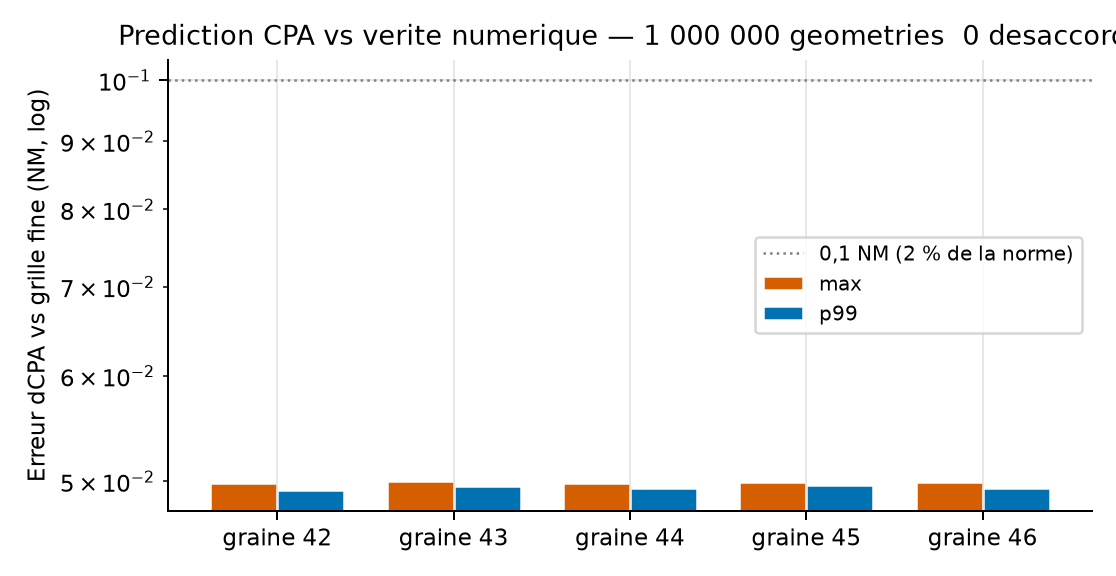
\includegraphics[width=0.68\textwidth]{figures/fig_cpa_multiseed.png}
\caption{Erreur de $d_{CPA}$ du prédicteur embarqué face à la grille numérique fine, par
graine (200\,000 géométries chacune). La décision de conflit est exacte : 0 désaccord sur
$10^6$ cas.}
\label{fig:cpa}
\end{figure}

\begin{figure}[t]
\centering
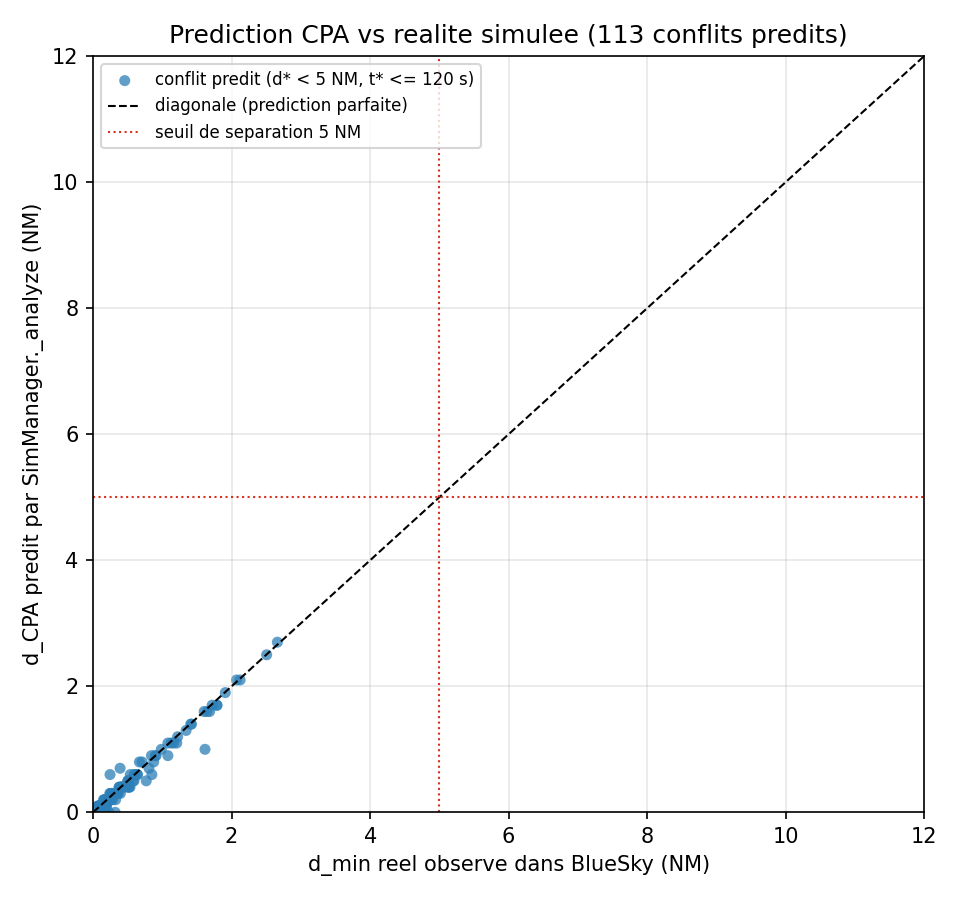
\includegraphics[width=0.62\textwidth]{figures/fig_bluesky_scatter.png}
\caption{$d_{CPA}$ prédit contre $d_{\min}$ mesuré dans BlueSky (200 rencontres) : MAE
0,067~NM, aucune erreur de classification (TP 113, FP 0, FN 0, TN 87).}
\label{fig:scatter}
\end{figure}

\begin{figure}[t]
\centering
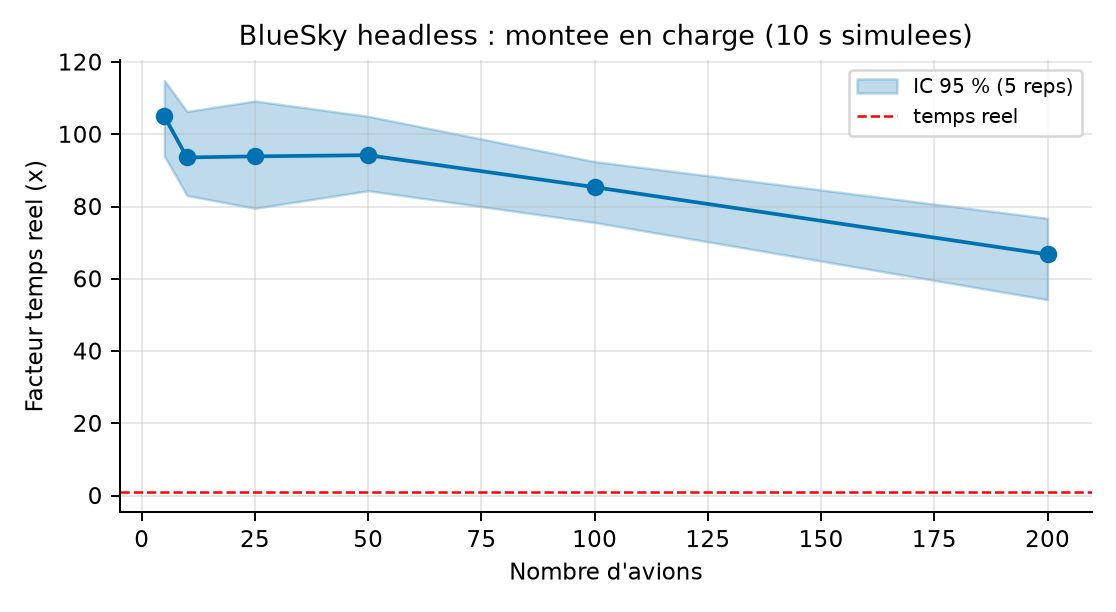
\includegraphics[width=0.66\textwidth]{figures/fig_sim_scaling.png}
\caption{Montée en charge de BlueSky headless (5 répétitions par point, IC bootstrap
95\,\%) : $\times$105 temps réel à 5 aéronefs, $\times$67 à 200. La simulation n'est
jamais le facteur limitant de la boucle vocale.}
\label{fig:scaling}
\end{figure}

\subsection{Reconnaissance vocale (STT)}
\label{sec:res-stt}

J'ai comparé cinq systèmes sur des échantillons ($n = 150$ par corpus, graine 42, décodage greedy) des deux corpus VHF \emph{réels}, avec mon protocole historique de normalisation et de WER (comparabilité avec les chiffres publiés en S4).

\begin{table}[h]
\centering
\small
\begin{tabular}{lcc}
\toprule
\rowcolor{lightgray}\textbf{Système (WER corpus, \%)} & \textbf{ATCO2-1h (hors domaine)} & \textbf{UWB-ATCC (test)}\\
\midrule
faster-whisper tiny & 100,9 & 120,1\\
faster-whisper base & 88,1 & 107,4\\
faster-whisper small & 71,5 & 92,3\\
whisper-small (vanilla) & 71,9 & 91,9\\
whisper-small + \textbf{LoRA ATC du projet} & \textbf{28,5} & \textbf{19,2}\\
\bottomrule
\end{tabular}
\caption{WER par système sur audio radio réel (condition passe-bande VHF de production
pour les systèmes small ; les WER supérieurs à 100\,\% traduisent un excès d'insertions
sur un domaine hors distribution). Détail, IC et conditions complètes :
\texttt{bench/results/stt\_bench.json}.}
\label{tab:stt}
\end{table}

J'en tire trois enseignements (figures~\ref{fig:sttwer} et \ref{fig:sttrtf}) :
\textbf{(i)} l'adaptation LoRA est le facteur dominant : le gain sur ATCO2 (domaine
jamais vu à l'entraînement) est d'environ 60\,\% relatif, confirmé par bootstrap apparié
($\Delta$WER $=-45$ points, IC 95\,\% $[-51 ; -40]$, excluant zéro), très loin devant tout
effet de taille de modèle ; \textbf{(ii)} le passe-bande VHF d'inférence améliore ou laisse
inchangé le modèle adapté (entraîné dans ce domaine), validant le choix de production ;
\textbf{(iii)} le déploiement local est réaliste : tous les systèmes tournent très en deçà
du temps réel sur GPU grand public (RTF 0,017 pour la voie LoRA). La valeur historique de
S4 (74,3 $\rightarrow$ 29,2\,\% sur le test ATCO2 complet) est retrouvée à un point près
par la re-mesure indépendante (71,9 $\rightarrow$ 28,5\,\% sur l'échantillon), ce qui
consolide les deux campagnes l'une par l'autre.

\begin{figure}[t]
\centering
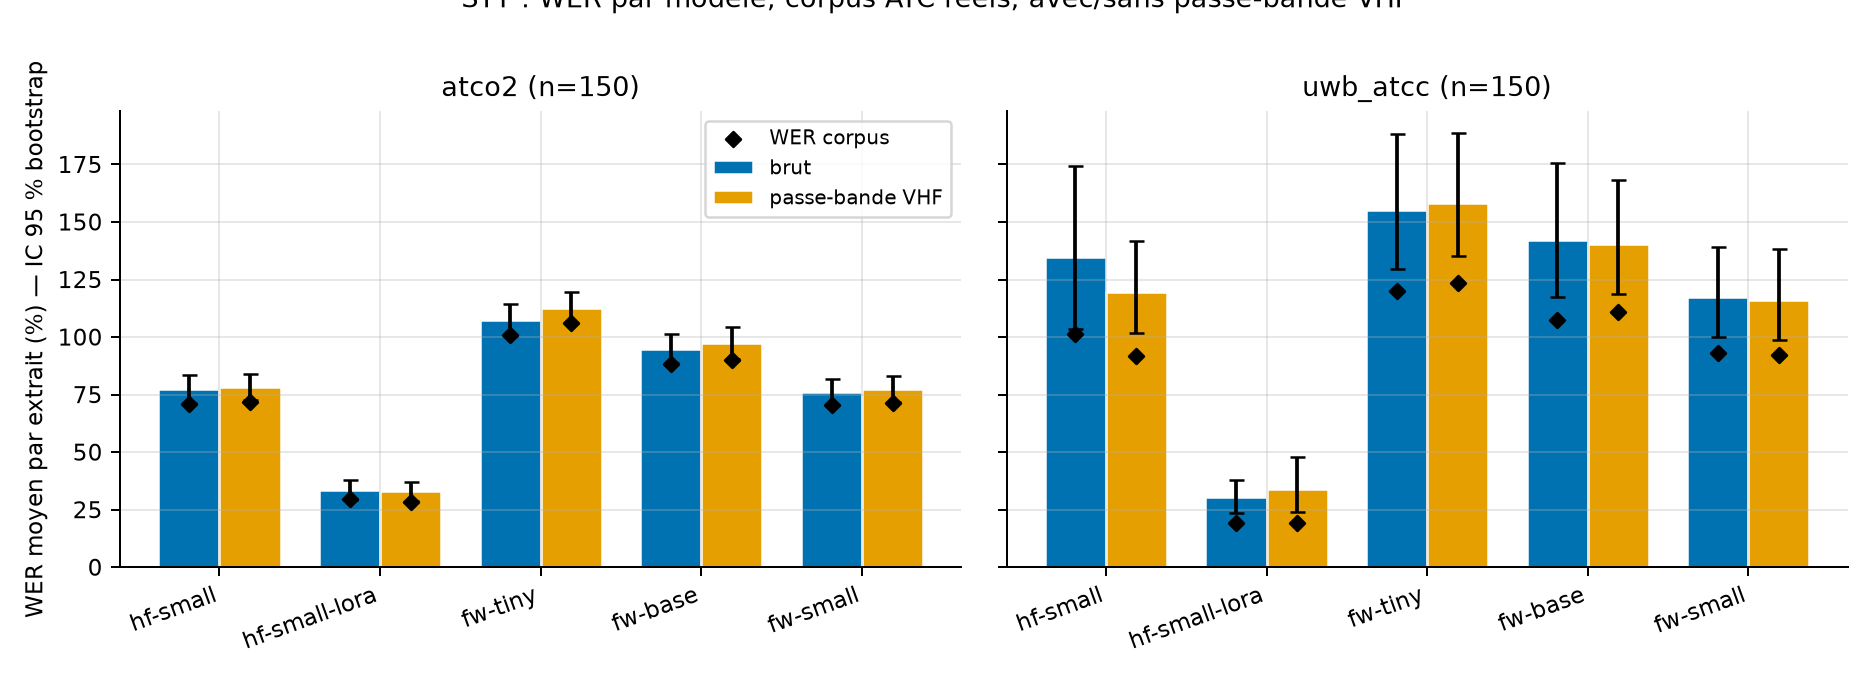
\includegraphics[width=0.95\textwidth]{figures/fig_stt_wer.png}
\caption{WER par système et par corpus (IC bootstrap 95\,\% du WER moyen par extrait ;
losanges : WER corpus).}
\label{fig:sttwer}
\end{figure}

\begin{figure}[t]
\centering

\includegraphics[width=0.7\textwidth]{figures/fig_stt_rtf.png}
\caption{Facteur temps réel de transcription (échelle log) : tous les systèmes sont
largement sous le temps réel sur GPU grand public.}
\label{fig:sttrtf}
\end{figure}

\subsection{Interprétation des clairances : comparaison appariée de quatre LLM et d'un parseur}
\label{sec:res-llm}

Mon corpus d'évaluation compte 116 clairances que j'ai annotées en TrafScript attendu \emph{après validation} : 68 cas dans la grammaire du parseur de référence et 48 cas étendus couvrant paraphrases hors grammaire, bruit de type STT (hésitations, répétitions), français parlé, nombres composés, multi-ordres et cas \emph{mixtes} (ordre valide $+$ ordre invalide dans la même phrase) ; le corpus compte 24 négatifs de sécurité au total. Un cas est réussi si le
multi-ensemble d'ordres produit est \emph{exactement} celui attendu. Tous les modèles
locaux sont quantifiés Q4\_K\_M et servis par llama.cpp à température 0.

\begin{table}[h]
\centering
\scriptsize
\begin{tabular}{l c c c c c c}
\toprule
\rowcolor{lightgray}\textbf{Système} & \textbf{Global [IC Wilson]} & \textbf{Dans gram.} & \textbf{Hors gram.} & \textbf{Négatifs rejetés} & \textbf{JSON strict} & \textbf{Latence moy.}\\
\midrule
Parseur à règles (réf.) & \textbf{87,9\,\%} [80,8 ; 92,7] & \textbf{100\,\%} & 70,8\,\% & 95,8\,\% & -- & $\sim$0,05~ms\\
Mistral-7B-v0.3 & \textbf{81,9\,\%} [73,9 ; 87,8] & 85,3\,\% & \textbf{77,1\,\%} & 75,0\,\% & 100\,\% & 0,82~s\\
Qwen2.5-1.5B & 75,0\,\% [66,4 ; 82,0] & 79,4\,\% & 68,8\,\% & 75,0\,\% & 96,6\,\% & \textbf{0,32~s}\\
Qwen2.5-3B & 24,1\,\% [17,3 ; 32,7] & 19,1\,\% & 31,3\,\% & 100\,\% & 45,7\,\% & 0,34~s\\
Qwen2.5-3B (bartowski) & 23,3\,\% [16,5 ; 31,7] & 20,6\,\% & 27,1\,\% & 95,8\,\% & 69,0\,\% & 0,42~s\\
Llama-3.2-1B & 3,4\,\% [1,3 ; 8,5] & 1,5\,\% & 6,3\,\% & 16,7\,\% & 22,4\,\% & 2,8~s\\
\bottomrule
\end{tabular}
\caption{Exactitude TrafScript exacte sur les 116 clairances, à travers la chaîne de
production complète (prompt + base OACI + validation déterministe). Source :
\texttt{bench/results/llm\_bench.json}.}
\label{tab:llm}
\end{table}

\noindent La lecture de ce tableau requiert les tests appariés (McNemar exact). Le résultat le plus important est une non-différence : entre le parseur et Mistral-7B, l'écart global n'est pas significatif ($n_{01} = 19$, $n_{10} = 12$, $p = 0{,}281$). La vraie différence est \emph{structurelle} : le parseur est parfait dans sa grammaire fermée (100\,\%) et s'effondre dehors (70,8\,\%), quand le LLM, légèrement moins bon dedans (85,3\,\%), est \emph{meilleur dehors} (77,1\,\%) ; c'est exactement l'écart qu'il était chargé de combler, et la raison pour laquelle je garde les deux, le parseur comme référence et oracle de test, le LLM en production. Les autres écarts sont nets : parseur contre Qwen2.5-1.5B, significatif ($p = 0{,}017$) ; contre Qwen-3B et Llama-1B, massivement significatif ($p < 10^{-20}$). Quant aux deux quantifications du Qwen-3B, elles sont indiscernables ($p = 1{,}0$) ; c'est le contrôle qui écarte l'artefact de conversion (\S\ref{sec:qwen}).

\noindent\textbf{Sécurité mesurée.} Même les petits modèles qui hallucinent des ordres sont
rattrapés par la validation déterministe : sur l'ensemble de la campagne, aucun ordre hors bornes ou hors schéma n'a été transmis au simulateur. Le taux de rejet des
négatifs par système (tableau~\ref{tab:llm}) chiffre la contribution de chaque couche, illustration directe de l'architecture de la section~\ref{sec:surete}.

\noindent\textbf{Point de fonctionnement.} Mistral-7B Q4 offre le meilleur compromis
qualité/latence locale (81,9\,\%, 0,8~s) ; étant le modèle servi sur ROMEO en bf16, il
fournit aussi la comparaison cluster/local. Qwen2.5-1.5B est le point << basse latence >>
exploitable (75\,\%, 0,32~s). Sur la tâche plus ouverte de génération de situations
(20 descriptions, 116 contraintes vérifiables), le générateur à règles reste à 100\,\%
contre 71,8\,\% pour le meilleur LLM : mon choix de production (génération géométrique locale, prouvée ; LLM pour le trafic d'ambiance) est confirmé.

\begin{figure}[t]
\centering
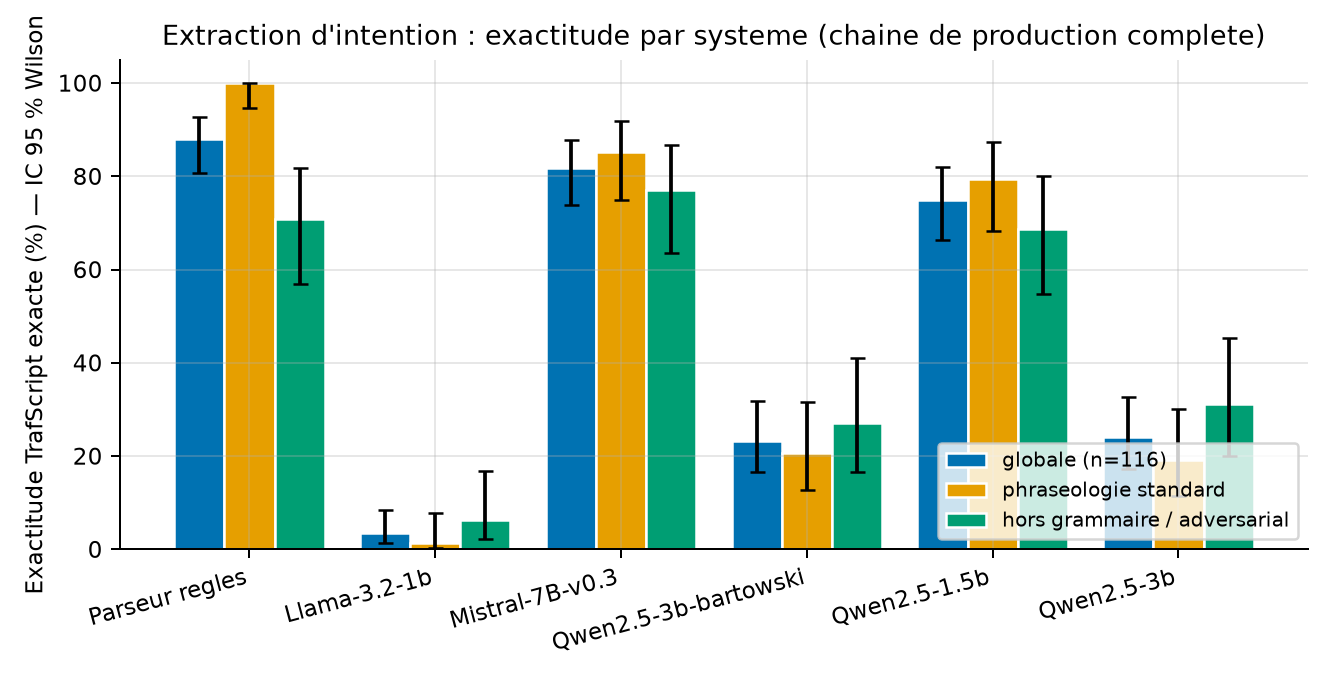
\includegraphics[width=0.95\textwidth]{figures/fig_llm_exactitude.png}
\caption{Exactitude par système (IC Wilson 95\,\%), globale et par strate : la
complémentarité parseur (grammaire fermée) / LLM (hors grammaire) est le résultat
structurant.}
\label{fig:llmacc}
\end{figure}

\begin{figure}[t]
\centering
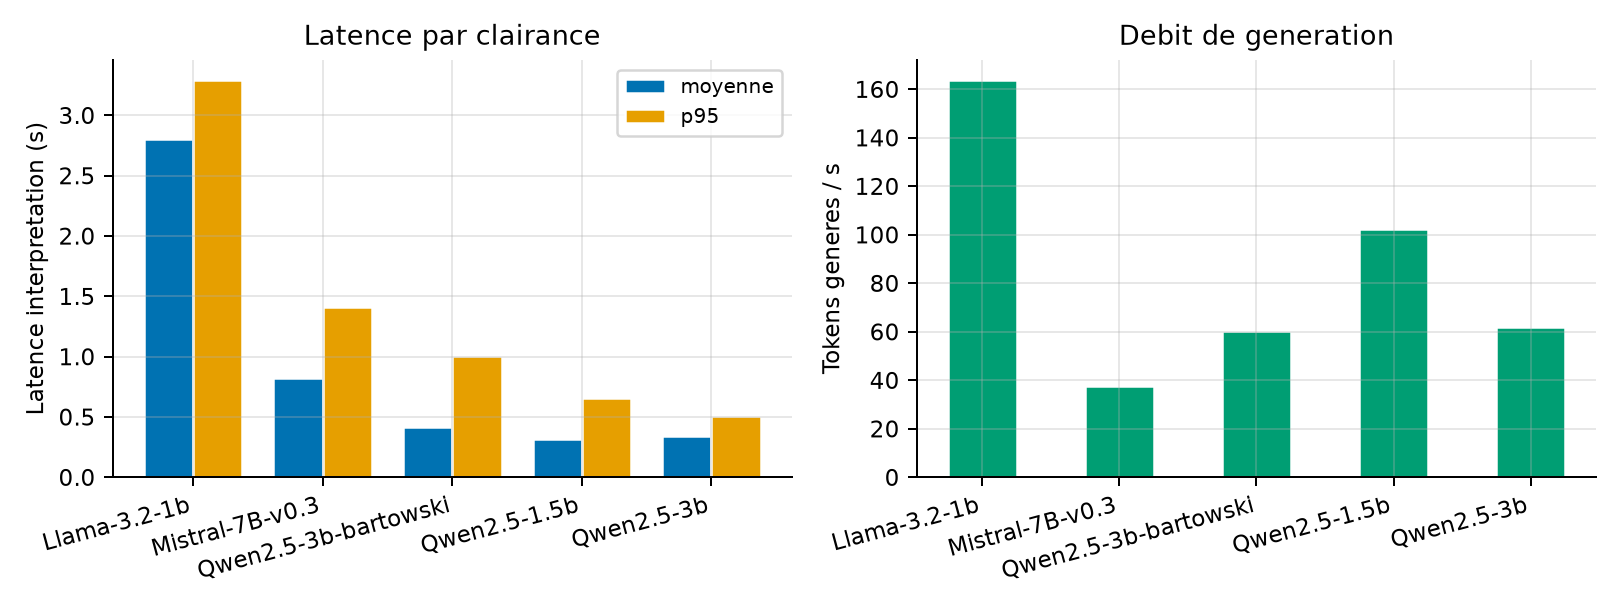
\includegraphics[width=0.95\textwidth]{figures/fig_llm_latence.png}
\caption{Latence d'interprétation et débit de génération des modèles locaux (RTX 4070,
llama.cpp Q4\_K\_M, température 0).}
\label{fig:llmlat}
\end{figure}

\subsection{Synthèse vocale}
\label{sec:res-tts}

Pour la synthèse vocale, j'ai fait passer à Kokoro-82M (4 voix) et à Windows SAPI le même exercice, 30 collationnements produits par mon générateur de phraséologie, jugés en coût (RTF) et en \emph{intelligibilité aller-retour} : le texte synthétisé est re-transcrit par un juge STT fixe et le WER
(normalisation sémantique symétrique : nombres épelés $\leftrightarrow$ chiffres) est
mesuré avant et après dégradation VHF. Kokoro synthétise à RTF 0,336 et son
intelligibilité aller-retour reste à 21,4\,\% \emph{après} canal VHF : la coloration radio
coûte peu d'intelligibilité, conformément à l'objectif (réalisme sans perte pédagogique).
La métrique partage le biais du juge entre moteurs : elle est \textbf{relative}, seuls les écarts entre systèmes sont interprétables, limite documentée dans le protocole. Sur le
cluster, la référence historique XTTS (voix clonées, CPU) reste 3,9~s par collationnement
avec un WER de re-transcription de 22--24\,\% mesuré par une métrique maison antérieure au
banc (non comparable au WER \texttt{jiwer}, et signalée comme telle).

\begin{figure}[t]
\centering
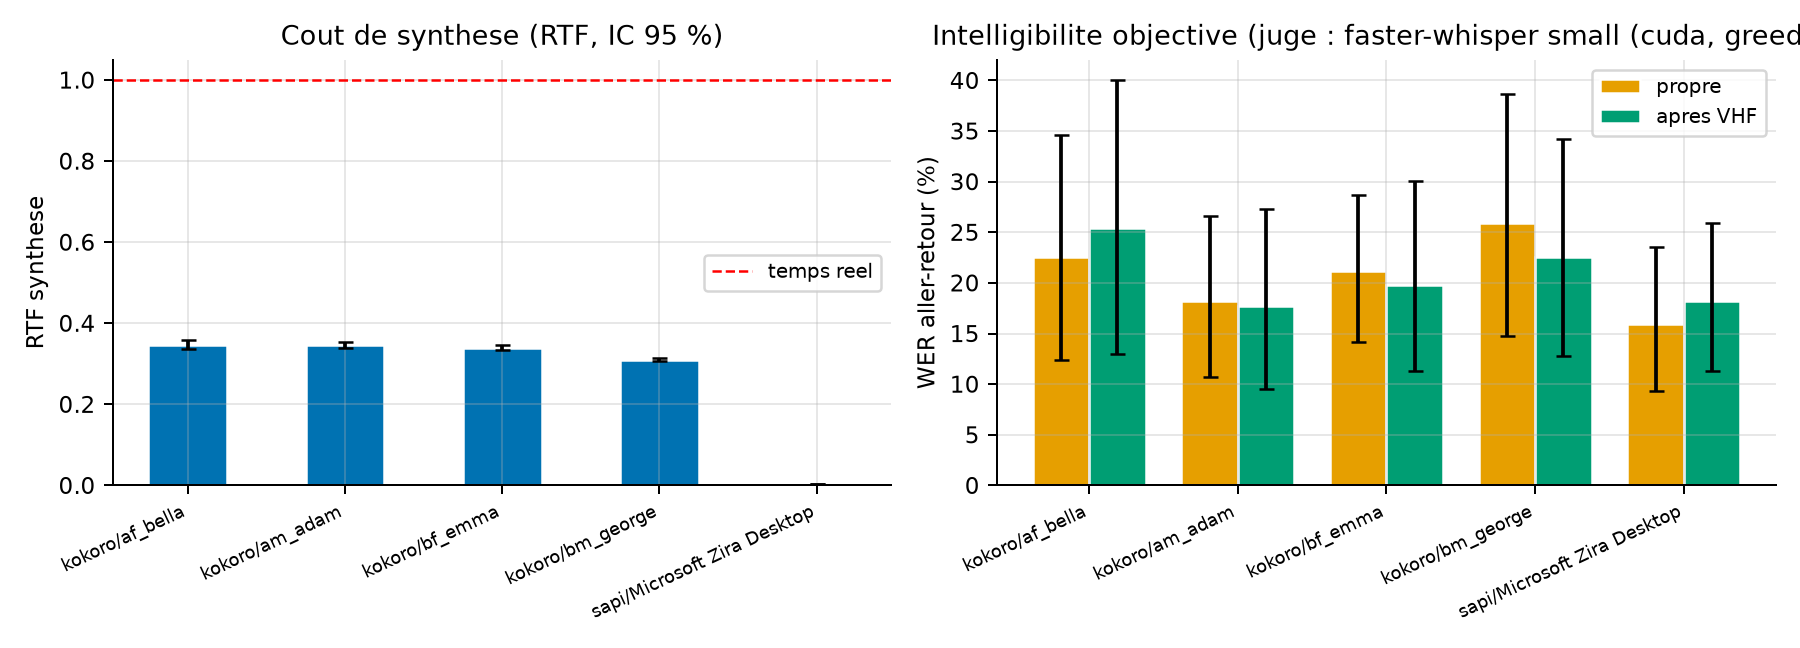
\includegraphics[width=0.95\textwidth]{figures/fig_tts.png}
\caption{Synthèse vocale : coût (RTF) et intelligibilité objective aller-retour,
avant/après canal VHF.}
\label{fig:tts}
\end{figure}

\subsection{La boucle vocale complète}
\label{sec:res-e2e}

Ma mesure finale répond à la question d'origine du stage : quand l'élève parle à un avion, celui-ci comprend-il, man\oe uvre-t-il et répond-il correctement ? Elle ferme la boucle de production entière sur 25 clairances \emph{parlées} : j'ai synthétisé chaque énoncé contrôleur par une voix jamais utilisée ailleurs dans le banc (SAPI), je l'ai fait passer dans un canal radio simulé (bruit SNR 12~dB puis passe-bande VHF), puis la chaîne complète a pris le relais : transcription par mon Whisper-LoRA, interprétation par Mistral-7B, validation, exécution, et collationnement en Kokoro dégradé VHF. Une condition témoin \emph{texte} (mêmes clairances, sans STT) isole le
coût de l'étage vocal.

\begin{table}[h]
\centering
\small
\begin{tabular}{lcc}
\toprule
\rowcolor{lightgray}\textbf{Boucle complète ($n=25$)} & \textbf{Condition voix} & \textbf{Témoin texte}\\
\midrule
Exécutions exactes & \textbf{76\,\%} (19/25), IC [56,6 ; 88,5] & 88\,\% (22/25), IC [70,0 ; 95,8]\\
Attribution des 6 échecs voix & 3 STT, 3 LLM, 0 fournisseur & --\\
\midrule
Latence STT / LLM / TTS (moy.) & 0,36~s / 1,06~s / 1,15~s & --\\
\textbf{Latence vocale totale} & \textbf{2,6~s} (p95 : 3,2~s) & --\\
\bottomrule
\end{tabular}
\caption{Boucle vocale de bout en bout sur GPU grand public
(\texttt{bench/results/e2e\_bench.json}). Référence cluster historique : ASR 0,84~s,
interprétation 5,2~s, TTS 3,9~s.}
\label{tab:e2e}
\end{table}

\begin{figure}[t]
\centering
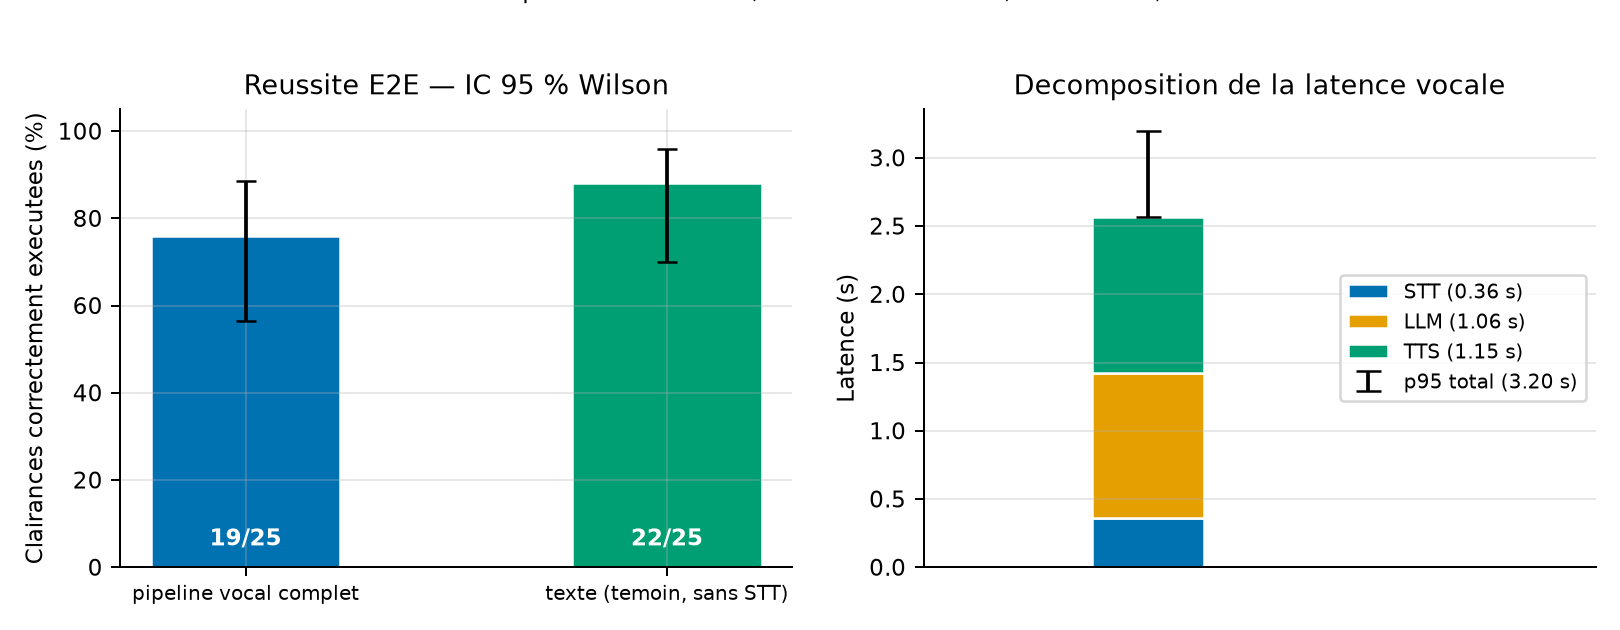
\includegraphics[width=0.95\textwidth]{figures/fig_e2e.png}
\caption{Boucle vocale complète : taux de réussite (voix contre témoin texte, IC Wilson)
et décomposition de la latence par étage.}
\label{fig:e2e}
\end{figure}

L'écart voix/texte (12 points) chiffre le coût résiduel de la reconnaissance vocale ; la latence totale de 2,6~s est compatible avec le rythme d'une fréquence d'entraînement (un échange toutes les 10--30~s). La figure~\ref{fig:romeo} montre la même boucle vérifiée sur le cluster dès la semaine 8 (descente FL280 $\rightarrow$ FL180 exécutée puis collationnée en voix clonée).

\paragraph{Contre-épreuve avec un locuteur humain réel.} La limite évidente de ce protocole restait la voix synthétique du contrôleur. Pour la lever, j'ai enregistré moi-même les 25 clairances au micro (capture par navigateur, le même chemin que le push-to-talk de l'application), en phraséologie parlée (indicatifs en téléphonie, chiffres épelés), puis je les ai passées dans la chaîne strictement identique, dans deux conditions : mes prises brutes, telles que l'application m'entend, et les mêmes prises dégradées par le canal radio du banc (bruit SNR 12~dB, même graine). Résultat : 20/25 (80\,\%, IC 95\,\% [60,9 ; 91,1]) en condition micro pour 2,3~s de latence moyenne, et 18/25 (72\,\%, IC [52,4 ; 85,7]) en condition radio, statistiquement indiscernable de la référence à voix synthétique. L'objectif premier du stage, parler aux avions et les entendre répondre, est donc vérifié avec un vrai locuteur, accent français compris. Le détail des échecs est instructif. Ma lecture en téléphonie réussit là où la lecture littérale de la voix SAPI échouait (EZY21, BAW57) ; en revanche l'indicatif << ryanair >> est systématiquement déformé par la transcription de ma voix (entendu << win air >>), et une clairance << reduce speed two five zero >> a été entendue << speed to five zero >>, produisant un ordre à 50~kt, dans les bornes physiques donc non filtré par les gardes. Le cas le plus révélateur : l'indicatif mixte épelé CSA1DZ est parfaitement transcrit (<< csa one delta zulu >>, WER 0) mais mal réassemblé par le LLM (CSAD12Z), exactement comme avec la voix synthétique ; ce défaut d'assemblage est indépendant du locuteur et désigne une amélioration précise, la normalisation déterministe des indicatifs épelés en amont du modèle. Protocole et résultats versionnés : \texttt{bench/human\_record\_web.py}, \texttt{bench/human\_e2e.py}, \texttt{bench/results/human\_e2e.json}.

\begin{figure}[t]
\centering
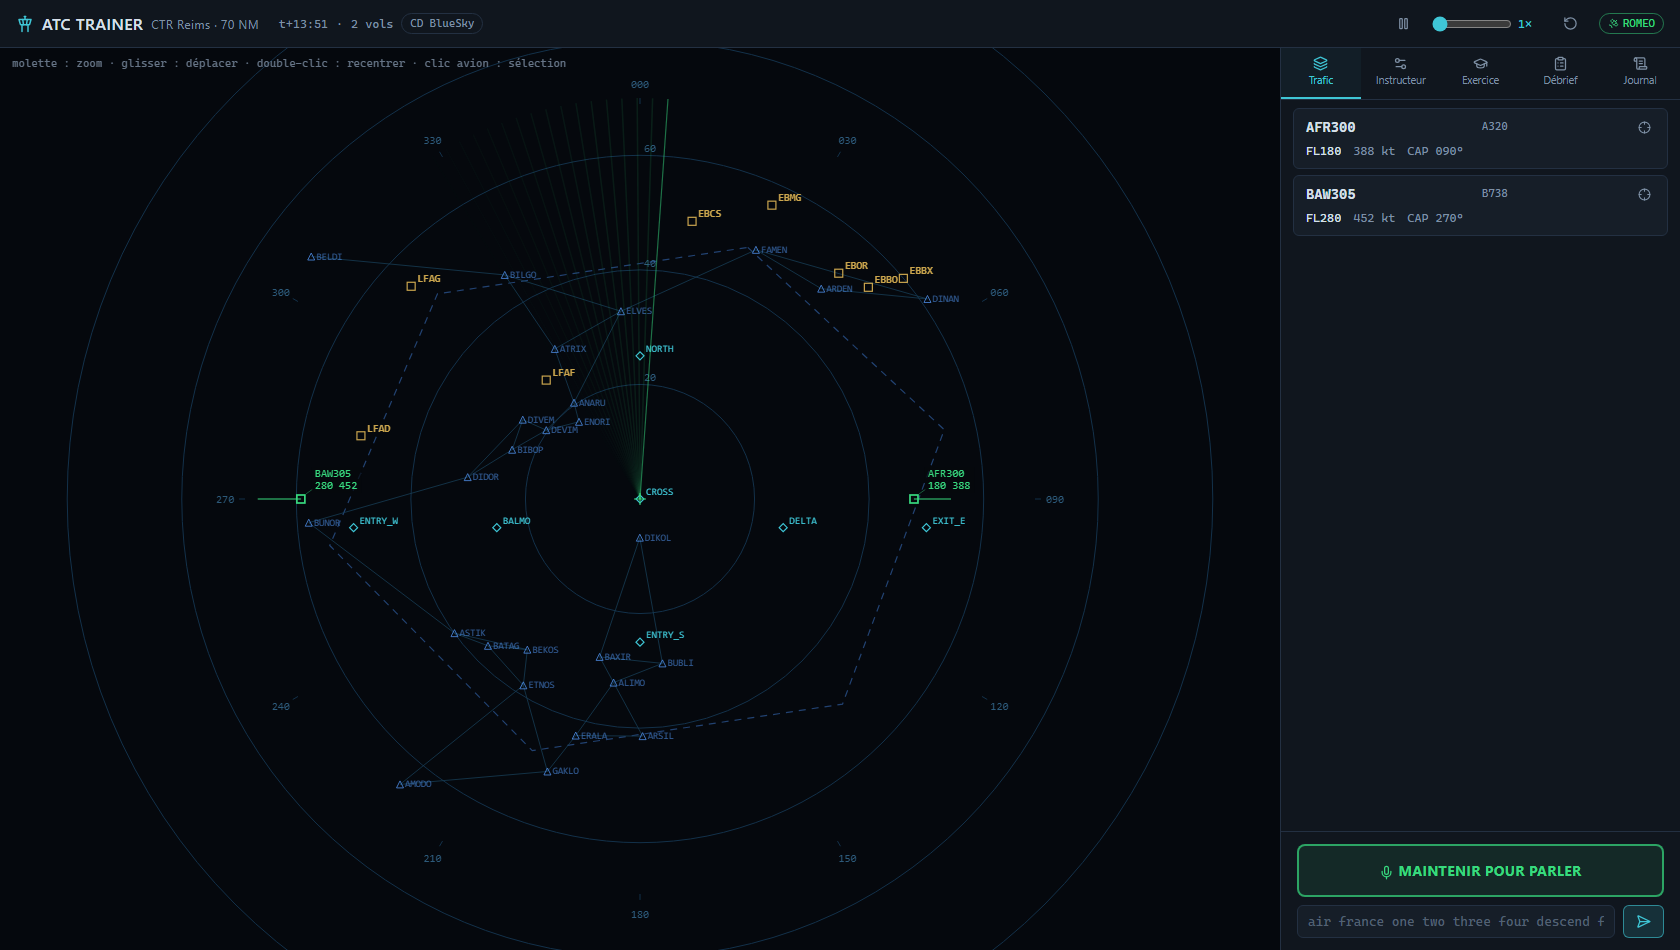
\includegraphics[width=0.88\textwidth]{figures/app_romeo.png}
\caption{La boucle vocale sur le cluster (semaine 8) : après une clairance parlée,
l'aéronef AFR300 est établi au FL180 et collationne dans sa voix clonée.}
\label{fig:romeo}
\end{figure}

\subsection{Reproductibilité}

Reste une question : que valent ces chiffres dans le temps ? Trois dispositifs les empêchent de devenir des instantanés invérifiables : \textbf{(i)} j'ai ré-exécuté intégralement la campagne de validation historique le 3 juillet : toutes les métriques sont identiques champ à champ aux JSON versionnés (seules les durées d'exécution diffèrent) ; \textbf{(ii)} j'ai muni \texttt{validation/run\_all.py} de portes de non-régression sur les métriques elles-mêmes (une chute de $F_1$ casse désormais l'exécution, réponse directe à une lacune relevée par mon audit) ;
\textbf{(iii)} l'intégralité du banc (scripts, corpus annotés, graines, JSON de résultats,
génération des figures et tableaux de l'article) est versionnée dans \texttt{bench/},
\texttt{validation/} et \texttt{docs/article/} du dépôt, et la suite de 209 tests
unitaires tourne en intégration continue.

%=============================================================================
\section{Limites et résultats négatifs}
\label{sec:limites}
%=============================================================================

Je recense ici, sans les minimiser, les limites et les résultats négatifs du projet, tous documentés dans le dépôt.

Côté modèles, deux échecs nets : Llama-3.2-1B est inutilisable sur la tâche (3,4\,\%) et Qwen2.5-3B viole le schéma de sortie (\S\ref{sec:qwen}) ; la génération de situations par LLM reste par ailleurs inférieure au générateur géométrique (71,8\,\% contre 100\,\%), en particulier sur les contraintes d'espacement. Ces résultats négatifs sont publiés avec leurs intervalles de confiance et, pour Qwen-3B, avec l'expérience de contrôle.

L'écart voix/texte demeure : 12 points de réussite séparent la boucle parlée du témoin texte ($n = 25$, IC larges), et la moitié des échecs vocaux vient de transcriptions déviées. Le WER de 28,5\,\% sur radio réelle, quoique divisé par 2,5, reste élevé pour un domaine critique. C'est la validation déterministe qui rend le système utilisable malgré ce taux, en convertissant les erreurs en rejets plutôt qu'en man\oe uvres erronées.

Mes mesures ont elles-mêmes leurs biais, que je connais. Les énoncés de la référence E2E sont synthétiques (voix SAPI + canal simulé) ; la contre-épreuve à locuteur humain réel (\S\ref{sec:res-e2e}) borne désormais ce biais, mais elle repose sur un seul locuteur, moi-même, en lecture et non en parole spontanée, sans la phraséologie fluide d'un professionnel ; les corpus réels couvrent par ailleurs ce risque pour l'étage STT isolé. L'intelligibilité TTS est une métrique relative (biais de juge partagé). Le WER historique << 22--24\,\% >> de la boucle XTTS utilisait une métrique maison non comparable à \texttt{jiwer}. Le corpus d'interprétation, quoique stratifié et adversarial, reste de taille modeste (116 cas) ; les IC de Wilson en tiennent compte.

La synthèse sur cluster n'est pas temps réel : XTTS reste confiné au CPU par le bug cuFFT du GH200 (3,9~s par collationnement), le correctif de compatibilité \texttt{transformers} est une dette technique explicite, et le point local (Kokoro, RTF 0,34) contourne le problème mais sans clonage de voix. Le périmètre simulé est lui aussi borné : secteur unique fictif centré sur Reims (7 points), hypothèse MRU sans vent pour le prédicteur (l'application transmet vitesse sol et route, mais la campagne de validation est à vent nul), pas de SID/STAR ni de 4D complet, application mono-poste locale sans authentification (exposition réseau hors périmètre).

Enfin, la traçabilité des chiffres de S4 était partielle : je n'avais pas versionné les artefacts d'entraînement (courbes, \texttt{train\_summary}), lacune que mon propre audit a relevée. C'est précisément ce qui m'a poussé à re-mesurer le LoRA au banc, de manière indépendante : la re-mesure retrouve les valeurs historiques à un point près et constitue désormais la référence traçable.

%=============================================================================
\section{Bilan}
%=============================================================================

\begin{resbox}[Ce que j'ai démontré à l'issue de ce stage]
\begin{itemize}
  \item \textbf{L'objectif premier est atteint : on peut parler aux avions, et ils répondent.} Parole $\rightarrow$ transcription adaptée au domaine $\rightarrow$ interprétation ancrée $\rightarrow$ validation déterministe $\rightarrow$ man\oe uvre dans le simulateur $\rightarrow$ collationnement vocal, à 76\,\% de réussite en voix synthétique et 80\,\% en contre-épreuve avec un locuteur humain réel, pour 2,6~s de latence sur GPU grand public, et vérifié sur cluster.
  \item \textbf{Des choix justifiés puis validés par la mesure} : chaque décision
  structurante (corpus, LoRA, LLM ancré non affiné, BlueSky, contrat OpenAI-compatible)
  est adossée à l'état de l'art, confrontée à ses alternatives, et confirmée a posteriori
  par une mesure versionnée (tableau~\ref{tab:decisions}).
  \item \textbf{Une base géométrique exacte} : $10^6$ décisions de conflit sans désaccord,
  $F_1 = 1{,}0$ face à BlueSky, conflits d'exercice garantis à 100\,\%.
  \item \textbf{Une sécurité qui ne dépend pas du modèle} : sur toute la campagne, aucun
  ordre hors bornes n'a atteint le simulateur, y compris avec les modèles les plus faibles.
  \item \textbf{Une démarche reproductible} : protocoles seedés, résultats JSON versionnés,
  ré-exécution identique champ à champ, 209 tests en CI, article de recherche dont chaque
  chiffre est généré depuis les données brutes.
\end{itemize}
\end{resbox}

Sur le plan des compétences, ce stage m'a fait parcourir le cycle complet d'un projet d'IA appliquée : la lecture critique de l'état de l'art et la sélection argumentée (jusqu'à écarter une approche publiée, l'affinage du LLM, pour des raisons de sécurité et de coût) ; l'ingénierie sous contraintes réelles (quota disque, architecture aarch64 exotique, bugs d'écosystème du niveau du gabarit de conversation ou de la DLL) ; la conception d'une architecture de sûreté en couches, et la découverte, par revue adversariale, qu'une de mes propres gardes était contournable ; et la construction d'un appareil de preuve (validation mathématique, campagne empirique, banc statistique apparié) qui distingue ce qui est démontré de ce qui est simplement plausible.

\medskip
\noindent\textbf{Ce que ce stage a changé dans ma façon de voir l'IA.} Je suis arrivé avec l'idée qu'un bon modèle fait un bon système ; je repars convaincu du contraire. Les épisodes qui m'ont le plus appris sont ceux où le modèle n'était pas en cause : un gabarit de conversation qui perd le message système, une comparaison de chaînes qui rend une garde contournable, un quota disque qui redessine tout un pipeline de données. J'en retire quelques certitudes méthodologiques. Un modèle ne s'évalue qu'à travers sa pile de déploiement réelle, jamais isolément. Dans un domaine où l'erreur a un coût, le déterminisme se place en aval de l'apprentissage : le LLM propose une interprétation, le code la vérifie, chacun fait ce qu'il sait faire. Et la mesure a cessé d'être à mes yeux une formalité de fin de projet ; c'est elle qui a trouvé mes bugs, arbitré mes choix et, au fond, écrit une bonne partie de ce rapport. Ces dix semaines m'ont aussi confirmé un goût personnel : celui de la preuve, plus encore que celui du prototype.

\medskip
\noindent\textbf{Perspectives.} Les suites naturelles sont l'injection de l'état de trafic courant dans la requête unifiée (conscience spatiale située), l'élargissement de la contre-épreuve humaine à plusieurs locuteurs, idéalement des contrôleurs ou élèves contrôleurs en phraséologie spontanée, et l'extension multi-secteurs.

\medskip
\noindent\textbf{Reproductibilité.} Code, corpus annotés, scripts de mesure, résultats
bruts et génération des figures : répertoires \texttt{bench/}, \texttt{validation/} et
\texttt{docs/article/} du dépôt GitHub du projet
(\texttt{Gotman08/} \texttt{simulateur-controleur-aerien}).

%=============================================================================
\begin{thebibliography}{99}\small

\bibitem{atco2} J.~Zuluaga-Gomez \emph{et al.}, << ATCO2 corpus: A Large-Scale Dataset for
Research on Automatic Speech Recognition and Natural Language Understanding of Air Traffic
Control Communications >>, arXiv:2211.04054, 2023.

\bibitem{uwbatcc} L.~Šmídl \emph{et al.}, << Air Traffic Control Communication (UWB-ATCC)
Corpus >>, Université de Bohême de l'Ouest, 2019.

\bibitem{atcosim} K.~Hofbauer, S.~Petrik et H.~Hering, << The ATCOSIM Corpus of
Non-Prompted Clean Air Traffic Control Speech >>, \emph{LREC}, 2008.

\bibitem{whisper} A.~Radford \emph{et al.}, << Robust Speech Recognition via Large-Scale
Weak Supervision >>, \emph{ICML}, 2023.

\bibitem{lora} E.~Hu \emph{et al.}, << LoRA: Low-Rank Adaptation of Large Language
Models >>, \emph{ICLR}, 2022.

\bibitem{vandoorn} J.~L.~P.~M. van Doorn, \emph{Applying Large-Scale Weakly Supervised
Automatic Speech Recognition to Air Traffic Control}, mémoire de master, TU Delft, 2023.

\bibitem{suhaq} J.~Su et O.~Haq, << Fine-Tuning Whisper for American English Air Traffic
Control Speech Recognition: A Data-Efficient Pipeline >>, Research Square,
doi:10.21203/rs.3.rs-8970162/v1, 2026.

\bibitem{zhang} Q.~Zhang et J.~H.~Mott, << An Exploratory Assessment of LLM's Potential
Toward Flight Trajectory Reconstruction Analysis >>, arXiv:2401.06204, 2024.

\bibitem{airtrafficgen} D.~Sid \emph{et al.}, << AirTrafficGen: Configurable Air Traffic
Scenario Generation with Large Language Models >>, arXiv:2508.02269, 2025.

\bibitem{sharifi} I.~Sharifi, A.~Zongo et P.~Wei, << Fine-Tuning Large Language Models for
Cooperative Tactical Deconfliction of Small Unmanned Aerial Systems >>, arXiv:2603.28561,
2026.

\bibitem{bluesky} J.~M. Hoekstra et J.~Ellerbroek, << BlueSky ATC Simulator Project: an
Open Data and Open Source Approach >>, \emph{ICRAT}, 2016.

\bibitem{mistral} A.~Q. Jiang \emph{et al.}, << Mistral 7B >>, arXiv:2310.06825, 2023.

\bibitem{qwen} Équipe Qwen, << Qwen2.5 Technical Report >>, arXiv:2412.15115, 2024.

\bibitem{xtts} E.~Casanova \emph{et al.}, << XTTS: a Massively Multilingual Zero-Shot
Text-to-Speech Model >>, \emph{INTERSPEECH}, 2024.

\bibitem{icao4444} OACI, \emph{Doc 4444 : Gestion du trafic aérien (PANS-ATM)},
16\textsuperscript{e} édition, 2016. (Source normative ; la base de connaissances du
projet est un contenu original, sans extrait verbatim.)

\end{thebibliography}

\end{document}
